%%%%%%%% ICML 2026 LATEX SUBMISSION FILE (PAPER DRAFT) %%%%%%%%%%%%%%%%%

\documentclass{article}

% Recommended packages for figures and better typesetting:
\usepackage{microtype}
\usepackage{multirow}
\usepackage{graphicx}
\usepackage{subcaption}
\usepackage{booktabs} % for professional tables
\usepackage{hyperref}
\usepackage{enumitem}

% Math + theorem tools:
\usepackage{amsmath}
\usepackage{amssymb}
\usepackage{mathtools}
\usepackage{amsthm}

\usepackage{placeins}

% Algorithms:
\usepackage{algorithm}
\usepackage{algorithmic}

% Citations:
\usepackage{natbib}

% If you use cleveref:
\usepackage[capitalize,noabbrev]{cleveref}

% Use the following line for the initial blind version submitted for review:
% \usepackage{icml2026}
% For preprint, use:
\usepackage[preprint]{icml2026}
% If accepted, instead use:
% \usepackage[accepted]{icml2026}

%%%%%%%%%%%%%%%%%%%%%%%%%%%%%%%%
% THEOREMS
%%%%%%%%%%%%%%%%%%%%%%%%%%%%%%%%
\theoremstyle{plain}
\newtheorem{theorem}{Theorem}[section]
\newtheorem{proposition}[theorem]{Proposition}
\newtheorem{lemma}[theorem]{Lemma}
\newtheorem{corollary}[theorem]{Corollary}
\theoremstyle{definition}
\newtheorem{definition}[theorem]{Definition}
\newtheorem{assumption}[theorem]{Assumption}
\theoremstyle{remark}
\newtheorem{remark}[theorem]{Remark}

% Todonotes (disable for camera-ready if desired):
\usepackage[textsize=tiny]{todonotes}

% Running title (short):
\icmltitlerunning{Co2PO: Coordinated Constrained Policy Optimization for Multi-Agent RL}

\begin{document}

\twocolumn[
\icmltitle{Co2PO: Coordinated Constrained Policy Optimization for Multi-Agent RL}

% Anonymous submission: do NOT include author info for initial submission.
\icmlsetsymbol{equal}{$\dagger$}

\begin{icmlauthorlist}
  \icmlauthor{Shrenik Patel}{equal,rutgers}
  \icmlauthor{Christine Truong}{equal,cmu}
\end{icmlauthorlist}

\icmlaffiliation{rutgers}{Rutgers University, New Brunswick, NJ}
\icmlaffiliation{cmu}{Carnegie Mellon University, Pittsburgh, PA}

\icmlcorrespondingauthor{Shrenik Patel}{shrenik.patel@rutgers.edu}
\icmlcorrespondingauthor{Christine Truong}{cmtruong@andrew.cmu.edu}

\icmlkeywords{Constrained Reinforcement Learning, Multi-Agent Reinforcement Learning, Communication, Safety}

\vskip 0.3in
]

\printAffiliationsAndNotice{\icmlEqualContribution}  % required (leave empty for blind)

\begin{abstract}
Constrained multi-agent reinforcement learning (MARL) faces a fundamental tension between exploration and safety-constrained optimization. Existing leading approaches, such as Lagrangian methods, typically rely on global penalties or centralized critics that react to violations after they occur, often suppressing exploration and leading to over-conservatism. We propose Co2PO, a novel MARL communication-augmented framework that enables coordination-driven safety through selective, risk-aware communication. Co2PO introduces a shared blackboard architecture for broadcasting positional intent and yield signals, governed by a learned hazard predictor that proactively forecasts potential violations over an extended temporal horizon. By integrating these forecasts into a constrained optimization objective, Co2PO allows agents to anticipate and navigate collective hazards without the performance trade-offs inherent in traditional reactive constraints. We evaluate Co2PO across a suite of complex multi-agent safety benchmarks, where it achieves higher returns compared to leading constrained baselines while converging to cost-compliant policies at deployment. Ablation studies further validate the necessity of risk-triggered communication, adaptive gating, and shared memory components.
\end{abstract}

%%%%%%%%%%%%%%%%%%%%%%%%%%%%%%%%%%%%%%%%%%%%%%%%%%%%%%%%%%%%%%%%%%%%%%%%%%%%%
\section{Introduction}
\label{sec:intro}

Constrained multi-agent reinforcement learning (MARL) aims to maximize collective return while satisfying safety constraints, but in cooperative settings this tension is especially sharp: aggressive exploration can incur costly violations, while overly conservative updates can prematurely suppress learning and prevent agents from discovering high-performing joint behavior \cite{brunke2022safelearning}. The problem is amplified by partial observability and interaction-driven dynamics. Even when agents share the same reward objective, safety failures often emerges from coordination breakdowns in timing, intent, or mutual awareness, rather than from conflicting incentives \cite{omidshafiei2015decentralizedcontrolpartiallyobservable, calzolari2026safeheterogeneousmultiagentrl}. As a result, purely reactive constraint handling can be slow to correct the underlying cause of violations, while heavy-handed penalties can make learning brittle \cite{brunke2022safelearning}.

We introduce Co2PO, a coordinated constrained policy optimization framework that targets these coordination-driven safety failures through \emph{selective, risk-aware coordination}. Rather than treating communication as a persistent channel, Co2PO uses it as a sparse control mechanism: agents write to a shared blackboard only when they predict elevated near-term hazard risk. Each write contains compact safety-relevant signals---a positional state summary, an intent vector, and a yield flag---that other agents can retrieve to condition their actions. This design preserves decentralized action selection while providing coordination signals precisely when interaction risk is most acute.

Across cooperative multi-agent safety benchmarks, Co2PO improves feasible performance and reaches cost-compliant policies at evaluation under the same training budget. We observe transient violations early in training, when hazard prediction and coordination behavior are still being learned, but final policies satisfy the cost constraint during evaluation. Our contributions are as follows:

\noindent\textbf{Contributions.}\par
\begin{itemize}\setlength\topsep{0pt}\setlength\itemsep{5pt}\setlength\parskip{0pt}\setlength\parsep{0pt}
  \item We introduce Co2PO, enabling selective coordination via a shared blackboard with decentralized actions.
  \item We propose hazard-triggered writes of compact signals (state, intent, yield) with adaptive write-rate control.
  \item We evaluate on cooperative multi-agent safety benchmarks with ablations isolating blackboard and gating.
\end{itemize}



%%%%%%%%%%%%%%%%%%%%%%%%%%%%%%%%%%%%%%%%%%%%%%%%%%%%%%%%%%%%%%%%%%%%%%%%%%%%%

%%%%%%%%%%%%%%%%%%%%%%%%%%%%%%%%%%%%%%%%%%%%%%%%%%%%%%%%%%%%%%%%%%%%%%%%%%%%%
\section{Problem Setup and Preliminaries}
\label{sec:setup}

We study constrained cooperative multi-agent reinforcement learning (MARL) under partial observability. Agents seek high return while satisfying an expected cost budget at evaluation, and we summarize performance with \emph{feasible return}.

\subsection{Constrained Cooperative Markov Game}
We model the environment as a cooperative constrained Markov game (CMG) with $n$ agents \cite{littman1994markovgames}:
\[
\mathcal{G} =
\langle
\mathcal{N}, \mathcal{S}, \{\mathcal{O}_i\}_{i\in\mathcal{N}},
\{\mathcal{A}_i\}_{i\in\mathcal{N}}, P, r, c, \gamma, \rho_0, d
\rangle .
\]
Agent $i$ observes $o_t^i\in\mathcal{O}_i$ and selects $a_t^i\in\mathcal{A}_i$, yielding joint action $a_t=(a_t^1,\dots,a_t^n)$ and transition $s_{t+1}\sim P(\cdot\mid s_t,a_t)$ from $s_0\sim\rho_0$.
The environment emits a shared reward $r_t=r(s_t,a_t)$ and safety cost $c_t=c(s_t,a_t)$.
% \footnote{When simulators provide per-agent costs, we enforce a team-level constraint using a standard aggregation (e.g., mean across agents).}

Policies factorize as $\pi(a\mid o)=\prod_{i=1}^n \pi_i(a^i\mid o^i)$ with $o=(o^1,\dots,o^n)$.
The discounted return and cost are
\begin{align}
J_R(\pi) &= \mathbb{E}_{\pi}\!\left[\sum_{t=0}^{\infty}\gamma^t\, r(s_t,a_t)\right], \label{eq:JR}\\
J_C(\pi) &= \mathbb{E}_{\pi}\!\left[\sum_{t=0}^{\infty}\gamma^t\, \bar{c}(s_t,a_t)\right], \label{eq:JC}
\end{align}
where $\bar{c}$ is the team cost used for enforcement.
We seek
\begin{equation}
\max_{\pi}\; J_R(\pi)\quad \text{s.t.}\quad J_C(\pi)\le d,
\label{eq:cmdg}
\end{equation}
with cost budget $d$.

\subsection{CTDE Preliminaries}
\label{sec:ctde}
We use centralized training with decentralized execution (CTDE): critics may condition on centralized information during training, while each actor $\pi_i$ conditions only on its local observation (and any permitted message/memory) at execution \cite{lowe2020multiagentactorcriticmixedcooperativecompetitive, yu2022surprisingeffectivenessppocooperative}.

\subsection{Safety Metric: Feasible Return}
\label{sec:safety-metrics}
We report \emph{feasible return} to reflect deployment-time cost constraints:
\begin{equation}
J_F(\pi) \;=\; J_R(\pi)\cdot \mathbf{1}\!\left[J_C(\pi)\le d\right].
\label{eq:feasible}
\end{equation}

\subsection{Lagrangian Relaxation}
\label{sec:lagrangian-prelims}
We optimize a Lagrangian relaxation of \cref{eq:cmdg}, following standard constrained policy optimization formulations \cite{achiam2017constrainedpolicyoptimization}:
\begin{equation}
\max_{\pi}\; \min_{\lambda\ge 0}\;\; \mathcal{L}(\pi,\lambda)
\;=\;
J_R(\pi)\;-\;\lambda\big(J_C(\pi)-d\big),
\label{eq:lagrangian}
\end{equation}
with the dual variable $\lambda$ updated online. Actor--critic updates commonly use a hybrid advantage \cite{tessler2018rcpo, ray2019safexp, zhang2020orderconstrainedoptimizationpolicy}
\begin{equation}
A^{\text{hyb}}_t \;=\; A^{R}_t \;-\; \lambda\, A^{C}_t.
\label{eq:hybrid-adv}
\end{equation}

\subsection{Risk Events and Hazard Labels}
\label{sec:hazard-labels}
We construct a proactive hazard label from dense per-step costs. Let $c_t^i$ be the instantaneous cost for agent $i$.
Define a hazard event
\begin{equation}
z_t^i \;=\; \mathbf{1}\!\left[c_t^i > \delta\right],
\label{eq:inst-hazard}
\end{equation}
and a lookahead label with horizon $H$,
\begin{equation}
h_t^i
\;=\;
\mathbf{1}\!\left[\max_{\tau \in \{t,\dots,t+H\}} z_\tau^i = 1\right],
\label{eq:lookahead-hazard}
\end{equation}
computed within episode boundaries. We use $h_t^i$ to supervise the hazard predictor used for selective coordination in \cref{sec:method}.


% \section{Problem Setup and Preliminaries}
% \label{sec:setup}

% We study \emph{constrained} cooperative multi-agent reinforcement learning (MARL), where agents must coordinate to maximize task return while satisfying safety constraints.
% We formalize the setting as a constrained Markov game under partial observability, and evaluate performance via \emph{feasible return} under a deployment-time cost budget.

% \subsection{Constrained Cooperative Markov Game}
% We consider a cooperative constrained Markov game (CMG) with $n$ agents,
% \[
% \mathcal{G} =
% \langle
% \mathcal{N}, \mathcal{S}, \{\mathcal{O}_i\}_{i\in\mathcal{N}},
% \{\mathcal{A}_i\}_{i\in\mathcal{N}}, P, r, c, \gamma, \rho_0, d
% \rangle .
% \]
% Here, $\mathcal{N}=\{1,\dots,n\}$ is the agent set, $\mathcal{S}$ is the global state space, and agent $i$ receives an observation $o_t^i \in \mathcal{O}_i$ at time $t$.
% Each agent selects an action $a_t^i \in \mathcal{A}_i$, inducing a joint action $a_t=(a_t^1,\dots,a_t^n)$ and next state $s_{t+1}\sim P(\cdot \mid s_t, a_t)$, with initial state $s_0 \sim \rho_0$.
% The environment provides a shared task reward $r_t = r(s_t, a_t)$ and a safety cost $c_t = c(s_t, a_t)$.\footnote{In our benchmarks, simulators may emit per-agent costs; we enforce constraints using a team-level aggregation (e.g., the mean across agents), consistent with standard cooperative safety evaluation.}


% Each agent has a stochastic policy $\pi_i(a^i\mid o^i)$ and the joint policy factorizes as
% $\pi(a\mid o)=\prod_{i=1}^n \pi_i(a^i\mid o^i)$, where $o=(o^1,\dots,o^n)$.
% We define the (discounted) return and cost of a joint policy $\pi$ as
% \begin{align}
% J_R(\pi) &= \mathbb{E}_{\pi}\!\left[\sum_{t=0}^{\infty}\gamma^t\, r(s_t,a_t)\right], \label{eq:JR}\\
% J_C(\pi) &= \mathbb{E}_{\pi}\!\left[\sum_{t=0}^{\infty}\gamma^t\, \bar{c}(s_t,a_t)\right], \label{eq:JC}
% \end{align}
% where $\bar{c}$ denotes the team cost used for constraint enforcement (e.g., team-average cost).
% The constrained objective is then
% \begin{equation}
% \max_{\pi}\; J_R(\pi)\quad \text{s.t.}\quad J_C(\pi)\le d,
% \label{eq:cmdg}
% \end{equation}
% with cost limit $d$.

% \subsection{CTDE Preliminaries}
% \label{sec:ctde}
% We adopt the centralized training and decentralized execution (CTDE) paradigm.
% During training, critics may condition on global information (e.g., centralized state or joint observations), while each actor $\pi_i$ conditions only on its local observation (and any permitted message/memory) at execution time.
% This separation is particularly important under partial observability, where coordination failures can induce safety violations even when each agent behaves reasonably from its local view.

% \subsection{Safety Metrics: Feasible Return and Deployment Safety}
% \label{sec:safety-metrics}
% We distinguish between (i) \emph{training-time} constraint satisfaction (which may be transiently violated during exploration) and (ii) \emph{deployment-time} safety of the learned policy under evaluation.
% Our primary claims focus on safe deployment: the final policy should meet the cost budget while achieving strong return.

% To summarize this tradeoff with a single scalar, we report \emph{feasible return}:
% \begin{equation}
% J_F(\pi) \;=\; J_R(\pi)\cdot \mathbf{1}\!\left[J_C(\pi)\le d\right],
% \label{eq:feasible}
% \end{equation}
% i.e., return is credited only if the evaluated policy is cost-compliant.

% % WE MAY HAVE TO REPORT THIS BUT IDK LETS SEE IF IT HELPS OUR CASE LOL!!
% % We also report cost curves and complementary safety statistics, including (i) violation rate (fraction of evaluation episodes exceeding the budget), (ii) time-to-feasible (steps until cost-compliance is reached and sustained), and (iii) peak/percentile costs to characterize transient risk.

% \subsection{Constrained Policy Optimization via Lagrangian Relaxation}
% \label{sec:lagrangian-prelims}
% A standard approach to constrained RL is to optimize a Lagrangian relaxation of \cref{eq:cmdg}:
% \begin{equation}
% \max_{\pi}\; \min_{\lambda\ge 0}\;\; \mathcal{L}(\pi,\lambda)
% \;=\;
% J_R(\pi)\;-\;\lambda\big(J_C(\pi)-d\big),
% \label{eq:lagrangian}
% \end{equation}
% where $\lambda$ is a dual variable updated online (primal--dual learning).
% In actor--critic implementations, the policy update commonly uses a \emph{hybrid advantage} that trades off reward and cost advantages:
% \begin{equation}
% A^{\text{hyb}}_t \;=\; A^{R}_t \;-\; \lambda\, A^{C}_t.
% \label{eq:hybrid-adv}
% \end{equation}
% While effective, purely reactive penalty updates can become conservative in multi-agent settings: early or interaction-driven violations may increase $\lambda$, suppressing exploration and slowing discovery of high-performing feasible behaviors.

% \subsection{Risk Events and Hazard Labels}
% \label{sec:hazard-labels}
% Beyond the episode-level budget in \cref{eq:cmdg}, many safety benchmarks provide dense per-step costs that indicate imminent risk (e.g., hazard proximity).
% We use these costs to define \emph{hazard events} and a \emph{proactive} supervision signal.

% Let $c_t^i$ denote the instantaneous cost attributed to agent $i$ at step $t$.
% We define an instantaneous hazard event as
% \begin{equation}
% z_t^i \;=\; \mathbf{1}\!\left[c_t^i > \delta\right],
% \label{eq:inst-hazard}
% \end{equation}
% where $\delta$ is a fixed threshold.
% To obtain a more proactive label with horizon $H$, we define a lookahead hazard indicator
% \begin{equation}
% h_t^i
% \;=\;
% \mathbf{1}\!\left[\max_{\tau \in \{t,\dots,t+H\}} z_\tau^i = 1\right],
% \label{eq:lookahead-hazard}
% \end{equation}
% computed within episode boundaries.
% Intuitively, $h_t^i$ marks whether agent $i$ will encounter a hazard within the next $H$ steps, and will serve as a risk signal for selective coordination (introduced in \cref{sec:method}).

% MAYBE PUT THIS IN APPENDIX?? DEPENDS ON ROOM, BUT COMMENTED OUT FOR NOW
% \subsection{Notation (Compact)}
% \label{sec:notation}
% \begin{table}[t]
% \caption{Compact notation used in \cref{sec:setup}.}
% \label{tab:notation}
% \centering
% \begin{small}
% \setlength{\tabcolsep}{4pt}
% \begin{tabular}{ll}
% \toprule
% Symbol & Meaning \\
% \midrule
% $n$ & number of agents \\
% $s_t,\; o_t^i,\; a_t^i$ & state, observation, action \\
% $r_t,\; c_t^i,\; \bar{c}_t$ & reward, per-agent cost, team cost \\
% $\gamma,\; d$ & discount, cost limit \\
% $J_R,\; J_C,\; J_F$ & return, cost, feasible return \\
% $\lambda$ & Lagrange multiplier \\
% $\delta,\; H$ & hazard threshold, lookahead horizon \\
% $z_t^i,\; h_t^i$ & instant / lookahead hazard indicators \\
% \bottomrule
% \end{tabular}
% \end{small}
% \vspace{-0.8em}
% \end{table}


%%%%%%%%%%%%%%%%%%%%%%%%%%%%%%%%%%%%%%%%%%%%%%%%%%%%%%%%%%%%%%%%%%%%%%%%%%%%%

%%%%%%%%%%%%%%%%%%%%%%%%%%%%%%%%%%%%%%%%%%%%%%%%%%%%%%%%%%%%%%%%%%%%%%%%%%%%%
\section{Methodology}
\label{sec:method}

We present Co2PO, a constrained MARL method that augments decentralized policies with \emph{selective} shared-memory coordination.
Each agent predicts near-term hazard risk from its local observation and writes a compact message to a shared blackboard only when predicted risk exceeds a threshold.
Agents then read a fixed-size context from the blackboard and condition their actions on the retrieved information.
Training uses a constrained actor--critic objective with reward and cost critics, a dual variable for constraint enforcement, supervised hazard forecasting, and a penalty that discourages excessive writing.

\subsection{Per-Timestep Interaction Protocol}
\label{sec:protocol}
We consider $E$ parallel environment instances and $n$ agents. At timestep $t$ in environment $e$:
\emph{(1) write-info} each agent computes hazard probability and message contents from its observation;
\emph{(2) write} agents gate writes and update the blackboard;
\emph{(3) read} each agent retrieves up to $k$ other agents' messages to form a fixed-length context;
\emph{(4) act} each agent selects an action conditioned on its observation and retrieved context.
The blackboard is maintained per environment instance and cleared on episode termination.

\subsection{Blackboard: State, Write, and Read}
\label{sec:blackboard}

\paragraph{Stored fields.}
For each environment $e$ and agent $i$, the blackboard stores a single current entry
\begin{equation}
B_t^{e,i} \;=\; \big(x_t^{e,i},\, u_t^{e,i},\, y_t^{e,i},\, p_t^{e,i},\, w_t^{e,i}\big),
\label{eq:blackboard-entry}
\end{equation}
where $x_t^{e,i}\in\mathbb{R}^{d}$ is a compact state summary,
$u_t^{e,i}\in\mathbb{R}^{d}$ is a learned intent vector,
$y_t^{e,i}\in[0,1]$ is a learned yield flag,
$p_t^{e,i}\in[0,1]$ is the hazard probability,
and $w_t^{e,i}\in\{0,1\}$ is the write indicator.

\paragraph{Write information from local observation.}
Each agent computes message fields and a hazard score from its observation:
\begin{equation}
(\ell_t^i,\; u_t^i,\; y_t^i) \;=\; F_\theta(o_t^i),
\qquad
p_t^i \;=\; \sigma(\ell_t^i),
\label{eq:write-info}
\end{equation}
where $\ell_t^i$ is a hazard logit and $\sigma(\cdot)$ is the sigmoid.

\paragraph{Event-triggered writes.}
Writes are gated by a threshold:
\begin{equation}
w_t^{e,i} \;=\; \mathbf{1}\!\left[p_t^{e,i} > \tau_t\right],
\label{eq:gate}
\end{equation}
and only entries with $w_t^{e,i}=1$ are valid for reads.

% \paragraph{Similarity-based read with fixed-length context.}
% Agent $i$ queries with $q_t^{e,i}=x_t^{e,i}$ and retrieves up to $k$ active entries by cosine similarity:
% \begin{align}
% s_t^{e}(i,j)
% &=
% \left\langle
% \frac{x_t^{e,j}}{\lVert x_t^{e,j}\rVert_2+\varepsilon},\;
% \frac{q_t^{e,i}}{\lVert q_t^{e,i}\rVert_2+\varepsilon}
% \right\rangle, \label{eq:cos-sim}\\
% \mathcal{K}_t^{e,i}
% &=
% \operatorname{TopK}_{\substack{j\neq i\\ w_t^{e,j}=1}}
% \Big(s_t^{e}(i,j)\Big),
% \label{eq:topk}
% \end{align}
% with $\varepsilon>0$.
% Each retrieved entry contributes
% \begin{equation}
% \psi\!\left(B_t^{e,j}\right)
% =
% \Big[x_t^{e,j}\,;\,u_t^{e,j}\,;\,y_t^{e,j}\,;\,p_t^{e,j}\Big]
% \in\mathbb{R}^{2d+2},
% \label{eq:psi}
% \end{equation}
% and agent $i$ forms a fixed-length context by concatenating up to $k$ vectors (zero-padded if fewer exist):
% \begin{equation}
% m_t^{e,i}
% =
% \Big[\psi(B_t^{e,j_1});\;\dots;\;\psi(B_t^{e,j_k})\Big]
% \in\mathbb{R}^{k(2d+2)}.
% \label{eq:memctx}
% \end{equation}

\paragraph{Similarity-based read (top-$k$) with fixed-length context.} At each timestep, agent $i$ forms a query vector from its own state summary, $q_t^{e,i}=x_t^{e,i}$.
It then considers the set of \emph{active} entries written by other agents in the same environment instance,
$\{\,B_t^{e,j}\,:\, j\neq i,\; w_t^{e,j}=1\,\}$, and scores each candidate $j$ by cosine similarity \cite{das2020tarmactargetedmultiagentcommunication}:
\[
s_t^{e}(i,j)=\left\langle
\frac{x_t^{e,j}}{\lVert x_t^{e,j}\rVert_2+\varepsilon},\;
\frac{q_t^{e,i}}{\lVert q_t^{e,i}\rVert_2+\varepsilon}
\right\rangle,
\]
where $\varepsilon>0$ is a small constant for numerical stability.
Agent $i$ retrieves the $k$ highest-scoring active entries and, for each retrieved sender $j$, constructs
\[
\psi(B_t^{e,j})=\big[x_t^{e,j};\,u_t^{e,j};\,y_t^{e,j};\,p_t^{e,j}\big]\in\mathbb{R}^{2d+2}.
\]
The memory context is the concatenation of up to $k$ such vectors in ranked order, zero-padded if fewer than $k$ entries are active:
\begin{equation}
m_t^{e,i}=\big[\psi(B_t^{e,j_1});\dots;\psi(B_t^{e,j_k})\big]\in\mathbb{R}^{k(2d+2)}.
\label{eq:memctx}
\end{equation}



\subsection{Threshold Control (Optional)}
\label{sec:adaptive-threshold}
We allow adaptation of $\tau_t$ online to target a desired write rate $\rho^\star$. Let $\rho_t$ be the observed mean write rate and $\bar{\rho}_t$ its exponential moving average \cite{stooke2020responsive}:
\begin{align}
\bar{\rho}_t &= \beta\,\bar{\rho}_{t-1} + (1-\beta)\,\rho_t, \label{eq:ema}\\
\tau_{t+1} &=
\operatorname{clip}\!\Big(\tau_t + \eta(\bar{\rho}_t-\rho^\star),\; \tau_{\min},\; \tau_{\max}\Big),
\label{eq:thr-update}
\end{align}
where $\beta\in(0,1)$, step size $\eta>0$, and bounds $(\tau_{\min},\tau_{\max})$ prevent degenerate write thresholds.

\subsection{Policy and Critics}
\label{sec:policy-critics}

\paragraph{Memory-conditioned decentralized actor.}
Each actor conditions on its observation and the retrieved context:
\begin{equation}
a_t^i \sim \pi_{\phi_i}\!\left(\cdot \mid o_t^i,\; \mathrm{enc}(m_t^i)\right),
\label{eq:actor}
\end{equation}
where $\mathrm{enc}(\cdot)$ maps \cref{eq:memctx} to an embedding concatenated with $o_t^i$.

\paragraph{Centralized critics.}
Under CTDE, we learn reward and cost critics $V^R(\cdot)$ and $V^C(\cdot)$ to compute reward and cost advantages for policy optimization.

\subsection{Learning Objective}
\label{sec:objective}

\paragraph{Constrained policy optimization.}
We optimize the Lagrangian objective (\cref{eq:lagrangian}) using a hybrid advantage
$A_t^{\text{hyb},i} = A_t^{R,i} - \lambda A_t^{C,i}$,
with $\lambda\ge 0$ updated by projected primal--dual learning.

\paragraph{Actor loss.}
Let $r_t^i(\phi_i)$ denote the importance ratio between current and behavior policies.
We use a clipped surrogate objective augmented with hazard supervision and a write penalty \cite{schulman2017proximalpolicyoptimizationalgorithms}:
\begin{equation}
\label{eq:actor-total}
\begin{aligned}
\mathcal{L}_{\text{actor}}^i
&=
\mathcal{L}_{\text{clip}}^i\!\left(A^{\text{hyb},i}\right)
+
\alpha_{\text{write}}\,
\mathbb{E}\!\left[w_t^i\right]
\\
&\quad
+
\alpha_{\text{haz}}\,
\mathbb{E}\!\left[
\operatorname{WBCE}\!\left(\ell_t^i,\; h_t^i\right)
\right]
-
\alpha_{\text{ent}}\,
\mathcal{H}\!\left(\pi_{\phi_i}\right).
\end{aligned}
\end{equation}
Here $\operatorname{WBCE}$ is weighted binary cross-entropy, $\mathcal{H}$ is policy entropy, and $\alpha_{\text{write}},\alpha_{\text{haz}},\alpha_{\text{ent}}\ge 0$ are coefficients.

% \paragraph{Hazard labels.}
% We supervise the hazard head using the lookahead label $h_t^i$ from \cref{sec:hazard-labels}.

% \paragraph{Critic losses and dual update.}
% Critics are trained by value regression against their respective returns. The dual variable $\lambda$ is updated with a projected step based on observed constraint violations.

\paragraph{Hazard supervision, critics, and dual update.}
We supervise the hazard head with the lookahead label $h_t^i$ (\cref{sec:hazard-labels}). Reward and cost critics are trained by value regression to their respective returns, and the dual variable $\lambda$ is updated via a projected step driven by observed constraint violations.


\subsection{Algorithm}
\label{sec:algorithm}

\begin{algorithm}[h!]
\caption{\textsc{Co2PO}: one rollout step at timestep $t$ (for all envs $e$ and agents $i$).}
\label{alg:co2po}
\begin{algorithmic}[1]
\STATE \textbf{Write-info:} compute $(\ell_t^{e,i},p_t^{e,i},u_t^{e,i},y_t^{e,i})$ from $o_t^{e,i}$ for all $(e,i)$
\STATE \textbf{Gate \& write:} set $w_t^{e,i} \leftarrow \mathbf{1}[p_t^{e,i}>\tau_t]$ and update blackboard entries $B_t^{e,i}$
\STATE \textbf{Adapt:} optionally update $\tau_t$ using \cref{eq:ema,eq:thr-update}
\STATE \textbf{Read:} for each $(e,i)$, form $m_t^{e,i}$ by top-$k$ retrieval from active entries (\cref{eq:memctx})
\STATE \textbf{Act:} sample $a_t^{e,i}\sim \pi_{\phi_i}(\cdot\mid o_t^{e,i}, \mathrm{enc}(m_t^{e,i}))$ and step environments
\STATE \textbf{Store:} add transitions (including $m_t^{e,i}$ and $w_t^{e,i}$) to buffer; clear blackboard for terminated envs
\end{algorithmic}
\end{algorithm}


% \section{Methodology}
% \label{sec:method}

% We present \textsc{Co2PO}, a constrained MARL method that augments decentralized policies with a \emph{selective} shared-memory communication mechanism.
% At a high level, each agent predicts near-term hazard risk from its local observation; only when this risk is high does the agent write a compact message to a shared blackboard.
% Agents then read a fixed-size context from the blackboard and condition their actions on this retrieved information.
% Training uses a constrained actor--critic objective with (i) reward and cost critics, (ii) a dual variable for constraint enforcement, (iii) supervised hazard forecasting, and (iv) an explicit penalty on writing.

% \subsection{Per-Timestep Interaction Protocol}
% \label{sec:protocol}

% We consider $E$ parallel environment instances (rollout threads) and $n$ agents.
% At each timestep $t$ and environment $e$, the interaction protocol proceeds in four stages:
% \emph{(1) write-info} each agent computes a hazard probability and message contents from its observation;
% \emph{(2) write} agents decide whether to write via a threshold gate and the blackboard is updated;
% \emph{(3) read} each agent retrieves up to $k$ other agents' messages to form a fixed-length context;
% \emph{(4) act} each agent selects an action conditioned on its observation and retrieved context.
% The blackboard is maintained \emph{per environment instance} and is cleared on episode termination for that instance.

% \subsection{Blackboard: State, Write, and Read}
% \label{sec:blackboard}

% \paragraph{Stored fields.}
% For each environment $e$ and agent $i$, the blackboard stores a single current entry
% \begin{equation}
% B_t^{e,i} \;=\; \big(x_t^{e,i},\, u_t^{e,i},\, y_t^{e,i},\, p_t^{e,i},\, w_t^{e,i}\big),
% \label{eq:blackboard-entry}
% \end{equation}
% where $x_t^{e,i}\in\mathbb{R}^{d}$ is a compact ``active'' state vector derived from the observation,
% $u_t^{e,i}\in\mathbb{R}^{d}$ is a learned \emph{intent} vector,
% $y_t^{e,i}\in[0,1]$ is a learned \emph{yield} flag,
% $p_t^{e,i}\in[0,1]$ is the hazard probability,
% and $w_t^{e,i}\in\{0,1\}$ is the write (active) indicator.

% \paragraph{Write information from local observation.}
% Each agent computes message fields and a hazard score from its local observation:
% \begin{equation}
% (\ell_t^i,\; u_t^i,\; y_t^i) \;=\; F_\theta(o_t^i),
% \qquad
% p_t^i \;=\; \sigma(\ell_t^i),
% \label{eq:write-info}
% \end{equation}
% where $\ell_t^i$ is a hazard logit, $\sigma(\cdot)$ is the sigmoid, and $F_\theta$ denotes lightweight prediction heads applied to $o_t^i$.

% \paragraph{Event-triggered writes.}
% The write indicator is computed via thresholding:
% \begin{equation}
% w_t^{e,i} \;=\; \mathbf{1}\!\left[p_t^{e,i} > \tau_t\right].
% \label{eq:gate}
% \end{equation}
% Only entries with $w_t^{e,i}=1$ are considered valid for other agents' reads.

% \paragraph{Similarity-based read with fixed-length context.}
% Agent $i$ queries the blackboard using $q_t^{e,i}=x_t^{e,i}$.
% Among other agents $j\neq i$ with $w_t^{e,j}=1$, it retrieves up to $k$ entries by cosine similarity:
% \begin{align}
% s_t^{e}(i,j)
% &=
% \left\langle
% \frac{x_t^{e,j}}{\lVert x_t^{e,j}\rVert_2+\varepsilon},\;
% \frac{q_t^{e,i}}{\lVert q_t^{e,i}\rVert_2+\varepsilon}
% \right\rangle, \label{eq:cos-sim}\\
% \mathcal{K}_t^{e,i}
% &=
% \operatorname{TopK}_{\substack{j\neq i\\ w_t^{e,j}=1}}
% \Big(s_t^{e}(i,j)\Big),
% \label{eq:topk}
% \end{align}
% with $\varepsilon>0$ for numerical stability.
% Each retrieved entry contributes the concatenation of the sender's state, intent, yield, and hazard score:
% \begin{equation}
% \psi\!\left(B_t^{e,j}\right)
% =
% \Big[x_t^{e,j}\,;\,u_t^{e,j}\,;\,y_t^{e,j}\,;\,p_t^{e,j}\Big]
% \in\mathbb{R}^{2d+2}.
% \label{eq:psi}
% \end{equation}
% The memory context for agent $i$ is the concatenation of up to $k$ such vectors, padding with zeros when fewer than $k$ valid entries exist:
% \begin{equation}
% m_t^{e,i}
% =
% \Big[\psi(B_t^{e,j_1});\;\dots;\;\psi(B_t^{e,j_k})\Big]
% \in\mathbb{R}^{k(2d+2)}.
% \label{eq:memctx}
% \end{equation}

% \subsection{Adaptive Threshold for Stable Write Rates}
% \label{sec:adaptive-threshold}

% The threshold $\tau_t$ in \cref{eq:gate} is updated online to track a target write rate $\rho^\star$.
% Let $\rho_t$ denote the observed mean write rate in the current batch (averaged over environments and agents).
% We maintain an exponential moving average $\bar{\rho}_t$ and update $\tau_t$ with a proportional controller:
% \begin{align}
% \bar{\rho}_t &= \beta\,\bar{\rho}_{t-1} + (1-\beta)\,\rho_t, \label{eq:ema}\\
% \tau_{t+1} &=
% \operatorname{clip}\!\Big(\tau_t + \eta(\bar{\rho}_t-\rho^\star),\; \tau_{\min},\; \tau_{\max}\Big),
% \label{eq:thr-update}
% \end{align}
% where $\beta\in(0,1)$, step size $\eta>0$, and bounds $(\tau_{\min},\tau_{\max})$ prevent degenerate thresholds.

% \subsection{Policy and Critics}
% \label{sec:policy-critics}

% \paragraph{Memory-conditioned decentralized actor.}
% Each agent's actor conditions on its local observation and the retrieved memory context:
% \begin{equation}
% a_t^i \sim \pi_{\phi_i}\!\left(\cdot \mid o_t^i,\; \mathrm{enc}(m_t^i)\right),
% \label{eq:actor}
% \end{equation}
% where $\mathrm{enc}(\cdot)$ is a small encoder that maps the fixed-length context in \cref{eq:memctx} to an embedding.
% The embedding is concatenated with the observation and passed through the policy network.

% \paragraph{Centralized critics.}
% Under CTDE, we learn a reward critic $V^R(\cdot)$ and a cost critic $V^C(\cdot)$ that can condition on centralized information.
% These critics provide reward and cost advantages $A_t^{R,i}$ and $A_t^{C,i}$ for policy optimization.

% \subsection{Learning Objective}
% \label{sec:objective}

% \paragraph{Constrained policy optimization.}
% We optimize a Lagrangian relaxation of the constrained objective (\cref{eq:cmdg}).
% The policy update uses the hybrid advantage
% $A_t^{\text{hyb},i} = A_t^{R,i} - \lambda A_t^{C,i}$,
% with $\lambda\ge 0$ updated via projected primal--dual learning.

% \paragraph{Actor loss.}
% Let $r_t^i(\phi_i)$ denote the importance ratio between the current and behavior policies.
% We use a clipped surrogate objective (PPO-style) with a hybrid advantage, augmented with supervised hazard forecasting and a write penalty:
% \begin{equation}
% \label{eq:actor-total}
% \begin{aligned}
% \mathcal{L}_{\text{actor}}^i
% &=
% \mathcal{L}_{\text{clip}}^i\!\left(A^{\text{hyb},i}\right)
% +
% \alpha_{\text{write}}\,
% \mathbb{E}\!\left[w_t^i\right]
% \\
% &\quad
% +
% \alpha_{\text{haz}}\,
% \mathbb{E}\!\left[
% \operatorname{WBCE}\!\left(\ell_t^i,\; h_t^i\right)
% \right]
% -
% \alpha_{\text{ent}}\,
% \mathcal{H}\!\left(\pi_{\phi_i}\right).
% \end{aligned}
% \end{equation}

% where $\operatorname{WBCE}$ is a weighted binary cross-entropy, $\mathcal{H}$ is policy entropy, and $\alpha_{\text{write}},\alpha_{\text{haz}},\alpha_{\text{ent}}\ge 0$ are coefficients.

% \paragraph{Hazard labels.}
% We supervise the hazard head with a lookahead hazard label $h_t^i$ (defined in \cref{sec:hazard-labels}) constructed from future per-step costs within the same episode.

% \paragraph{Critic losses and dual update.}
% Reward and cost critics are trained by value regression against their respective returns (using a robust regression loss).
% The dual variable $\lambda$ is updated with a projected step that increases penalty weight when observed episode costs exceed the budget, incorporating both episodic cost deviation and on-policy cost advantages.

% \subsection{Algorithm}
% \label{sec:algorithm}

% \begin{algorithm}[h!]
% \caption{\textsc{Co2PO}: one rollout step at timestep $t$ (for all envs $e$ and agents $i$).}
% \label{alg:co2po}
% \begin{algorithmic}[1]
% \STATE \textbf{Write-info:} compute $(\ell_t^{e,i},p_t^{e,i},u_t^{e,i},y_t^{e,i})$ from $o_t^{e,i}$ for all $(e,i)$
% \STATE \textbf{Gate \& write:} set $w_t^{e,i} \leftarrow \mathbf{1}[p_t^{e,i}>\tau_t]$ and update blackboard entries $B_t^{e,i}$
% \STATE \textbf{Adapt:} update $\tau_t$ using \cref{eq:ema,eq:thr-update} (optional)
% \STATE \textbf{Read:} for each $(e,i)$, form $m_t^{e,i}$ by top-$k$ retrieval from active entries (\cref{eq:topk,eq:memctx})
% \STATE \textbf{Act:} sample $a_t^{e,i}\sim \pi_{\phi_i}(\cdot\mid o_t^{e,i}, \mathrm{enc}(m_t^{e,i}))$ and step environments
% \STATE \textbf{Store:} add transitions (including $m_t^{e,i}$ and $w_t^{e,i}$) to buffer; clear blackboard for terminated envs
% \end{algorithmic}
% \end{algorithm}




%%%%%%%%%%%%%%%%%%%%%%%%%%%%%%%%%%%%%%%%%%%%%%%%%%%%%%%%%%%%%%%%%%%%%%%%%%%%%

%%%%%%%%%%%%%%%%%%%%%%%%%%%%%%%%%%%%%%%%%%%%%%%%%%%%%%%%%%%%%%%%%%%%%%%%%%%%%%
\section{Experimental Setup}
\label{sec:experiments}

\subsection{Benchmarks}
We evaluate on cooperative multi-agent safety benchmarks from the \textsc{SafePO} suite, which builds on \textsc{Safety-Gymnasium} and provides a consistent multi-agent interface \citep{ji2024safetygymnasiumunifiedsafereinforcement}.
Each task emits a per-step reward and safety cost; our goal is to maximize return while meeting an episodic cost budget.

\paragraph{Velocity family.}
In multi-agent velocity tasks, agents must coordinate to achieve velocity-tracking objectives while avoiding unsafe behavior under task-specific safety costs \citep{6386109}.
These tasks are coordination-stressing because agents share a space: one agent’s behavior can perturb others’ motion, making it harder to maintain target speeds without constraint violations.

\paragraph{MultiGoal family.}
In multi-agent MultiGoal tasks, agents navigate shared spaces with safety costs arising from unsafe states or contacts (e.g., hazards) \citep{ji2024safetygymnasiumunifiedsafereinforcement}.
They stress partial observability, interaction-driven hazards, and implicit negotiation to remain cost-compliant.

\subsection{Baselines}
We compare against constrained MARL baselines implemented in \textsc{SafePO}: \emph{MAPPO} \cite{yu2022surprisingeffectivenessppocooperative}, \emph{HAPPO} \cite{kuba2022happo}, \emph{MACPO} \cite{gu2023macpo}, and \emph{MAPPO-Lagrangian} \cite{gu2023macpo}.
All methods are run under a matched training budget and evaluation protocol. When available, we use \textsc{SafePO}'s standard hyperparameter configurations for each baseline and environment to avoid unfair retuning. All hyperparameters for all methods (including method-specific settings) are reported in Appendix \ref{app:hparams} for reproducibility.

\subsection{Metrics}
Let an episode have horizon $T$ with $n$ agents.
Following the \textsc{SafePO} convention, we aggregate reward and cost across agents by averaging per-step signals over agents and summing over time:
\begin{align}
R \;=\; \sum_{t=0}^{T-1}\frac{1}{n}\sum_{i=1}^n r_t^i,
\qquad
C \;=\; \sum_{t=0}^{T-1}\frac{1}{n}\sum_{i=1}^n c_t^i.
\label{eq:episodic-return-cost}
\end{align}
We evaluate policies at checkpoints $t\in\mathcal{T}$ during training; let $\widehat{R}_t,\widehat{C}_t$ denote mean episodic return/cost over evaluation episodes at checkpoint $t$.
We report:
\begin{itemize}\setlength\itemsep{2pt}\setlength\parskip{0pt}\setlength\parsep{0pt}\setlength\topsep{2pt}
  \item \textbf{Final return/cost} ($R_{\text{final}},C_{\text{final}}$): $\widehat{R}_{t_{\text{last}}}$ and $\widehat{C}_{t_{\text{last}}}$ at the last checkpoint $t_{\text{last}}$.
  \item \textbf{Peak cost} ($C_{\text{peak}}$): $\max_{t\in\mathcal{T}}\widehat{C}_t$, capturing the worst evaluated cost over training.
  \item \textbf{Violation rate}: fraction of evaluation episodes whose episodic cost exceeds the budget $d$ (i.e., $\Pr[C>d]$).
  \item \textbf{Feasible return} ($R_{\mathrm{feas}}$): best evaluation return among checkpoints that satisfy the cost budget,
  \begin{equation}
    R_{\mathrm{feas}} \;=\; \max_{t \in \mathcal{T}}\Big\{\widehat{R}_t \;:\; \widehat{C}_t \le d\Big\}.
    \label{eq:feasible-return}
  \end{equation}
  \item \textbf{Time-to-feasible}: the earliest training step corresponding to a checkpoint $t$ with $\widehat{C}_t \le d$; if no checkpoint is feasible, we report ``--''.
\end{itemize}

\subsection{Training and Evaluation Protocol}
We follow the standard \textsc{SafePO} on-policy training loop: collect rollouts with $E$ parallel environment instances, perform multiple epochs of minibatch updates per iteration, and periodically evaluate the current policy in separate evaluation rollouts \citep{ji2024safetygymnasiumunifiedsafereinforcement}.
Evaluation uses deterministic action selection and reports means (± standard deviation) over three independent random seeds.


% \section{Experimental Setup}
% \label{sec:experiments}

% \subsection{Benchmarks}
% We evaluate on multi-agent safety benchmarks provided by the \textsc{SafePO} suite, which builds on the \textsc{Safety-Gymnasium} environments and exposes a consistent multi-agent MuJoCo-style interface \citep{pku_safepo,ray2022rllib,tianshou,safety_gymnasium}.
% All tasks provide a per-step reward signal and a per-step safety cost signal; the learning objective is to maximize return while keeping expected episodic cost below a fixed budget.

% \paragraph{Velocity family.}
% In \emph{multi-agent velocity} tasks, agents must coordinate to achieve velocity-tracking objectives while avoiding unsafe behavior under environment-specific safety thresholds (e.g., velocity thresholds for different agent configurations) \citep{safety_gymnasium}.
% These tasks are particularly coordination-stressing because collisions, blocking, and interaction-induced dynamics can increase risk even when each agent acts myopically safe.

% \paragraph{MultiGoal family.}
% In \emph{multi-agent MultiGoal} tasks, agents must reach goals in shared spaces where safety costs arise from unsafe states or contacts (e.g., hazards) \citep{safety_gymnasium}.
% These environments stress (i) partial observability, (ii) interaction-driven hazards, and (iii) the need for implicit negotiation (e.g., yielding/right-of-way) to remain cost-compliant.

% \subsection{Baselines}
% We compare against representative constrained MARL baselines implemented in \textsc{SafePO}:
% \emph{MAPPO}, \emph{HAPPO}, \emph{MACPO}, and \emph{MAPPO-Lagrangian} \citep{pku_safepo}.
% All methods are run under a matched training budget and evaluation protocol.
% When available, we use the standard \textsc{SafePO} hyperparameter configurations for each environment and baseline to avoid unfair retuning.
% A full hyperparameter table for all methods (including method-specific settings) is provided in the appendix.

% \subsection{Metrics}
% Let an episode have horizon $T$ with $n$ agents.
% We report metrics computed from the \textsc{Safety-Gymnasium}/\textsc{SafePO} reward and cost signals, aggregated at the episode level.
% Following the common reporting convention in the \textsc{SafePO} pipeline, we aggregate across agents by averaging per-step signals over agents and summing over time:
% \begin{align}
% R \;=\; \sum_{t=0}^{T-1}\frac{1}{n}\sum_{i=1}^n r_t^i,
% \qquad
% C \;=\; \sum_{t=0}^{T-1}\frac{1}{n}\sum_{i=1}^n c_t^i.
% \label{eq:episodic-return-cost}
% \end{align}
% We use the following evaluation metrics:\vspace{-0.25em}
% \begin{itemize}\setlength\itemsep{8pt}\setlength\parskip{0pt}\setlength\parsep{0pt}\setlength\topsep{2pt}
%   \item \textbf{Episode return} ($\mathbb{E}[R]$): mean episodic return over evaluation episodes.
%   \item \textbf{Episode cost} ($\mathbb{E}[C]$): mean episodic cost over evaluation episodes.
%   \item \textbf{Violation rate}: fraction of evaluation episodes with episodic cost exceeding the budget $d$, i.e., $\Pr[C>d]$.
%   \item \textbf{Tail/peak cost}: high-percentile (e.g., 95th) and maximum episodic cost across evaluation episodes.
%   \item \textbf{Feasible return}: best evaluation return among checkpoints that satisfy the cost budget,
%   \begin{equation}
%     R_{\mathrm{feas}} \;=\; \max_{t \in \mathcal{T}}\Big\{\widehat{R}_t \;:\; \widehat{C}_t \le d\Big\},
%     \label{eq:feasible-return}
%   \end{equation}\vspace{-0.1em}
%   where $\widehat{R}_t,\widehat{C}_t$ are evaluation estimates at checkpoint $t$.
%   \item \textbf{Time-to-feasible}: earliest checkpoint at which the evaluated policy becomes cost-compliant (and remains compliant under smoothing).
% \end{itemize}

% \subsection{Training and Evaluation Protocol}
% We follow the standard \textsc{SafePO} training loop: collect on-policy rollouts with $E$ parallel environment instances, perform multiple epochs of minibatch updates per iteration, and periodically evaluate the current policy in separate evaluation rollouts \citep{pku_safepo}.
% Evaluation uses deterministic action selection and reports mean episodic return and cost across a fixed number of evaluation episodes and multiple random seeds.
% Unless otherwise stated, we plot learning curves with the mean across seeds and report variability (standard deviation or standard error) in shaded regions.

% \subsection{Compute and Key Hyperparameters}
% Table~\ref{tab:exp-hparams} lists the key shared hyperparameters that define the training budget and constraint setting.
% We follow \textsc{SafePO}'s standard defaults for these values unless explicitly overridden for a given environment \citep{pku_safepo}.
% All remaining hyperparameters (including method-specific communication settings and any environment-specific overrides) are reported in the appendix for full reproducibility.

% \begin{table}[h!]
%   \caption{Key experimental hyperparameters (shared across methods unless noted).}
%   \label{tab:exp-hparams}
%   \centering
%   \begin{small}
%   \setlength{\tabcolsep}{6pt}
%   \begin{tabular}{l c}
%     \toprule
%     \textbf{Setting} & \textbf{Value} \\
%     \midrule
%     Total environment steps ($N$) & $3\times 10^{7}$ \\
%     Episode horizon ($T$) & $1000$ \\
%     Rollout threads ($E$) & $10$ \\
%     Discount ($\gamma$) & $0.99$ \\
%     Cost budget ($d$) & $25$ \\
%     Actor learning rate & $5\times 10^{-4}$ \\
%     Critic learning rate & $5\times 10^{-4}$ \\
%     Initial dual variable ($\lambda_0$) & $0.1$ \\
%     Dual step size & $5\times 10^{-4}$ \\
%     \bottomrule
%   \end{tabular}
%   \end{small}
%   \vskip -0.08in
% \end{table}

%%%%%%%%%%%%%%%%%%%%%%%%%%%%%%%%%%%%%%%%%%%%%%%%%%%%%%%%%%%%%%%%%%%%%%%%%%%%%
\begin{figure*}[h!]
  \centering
  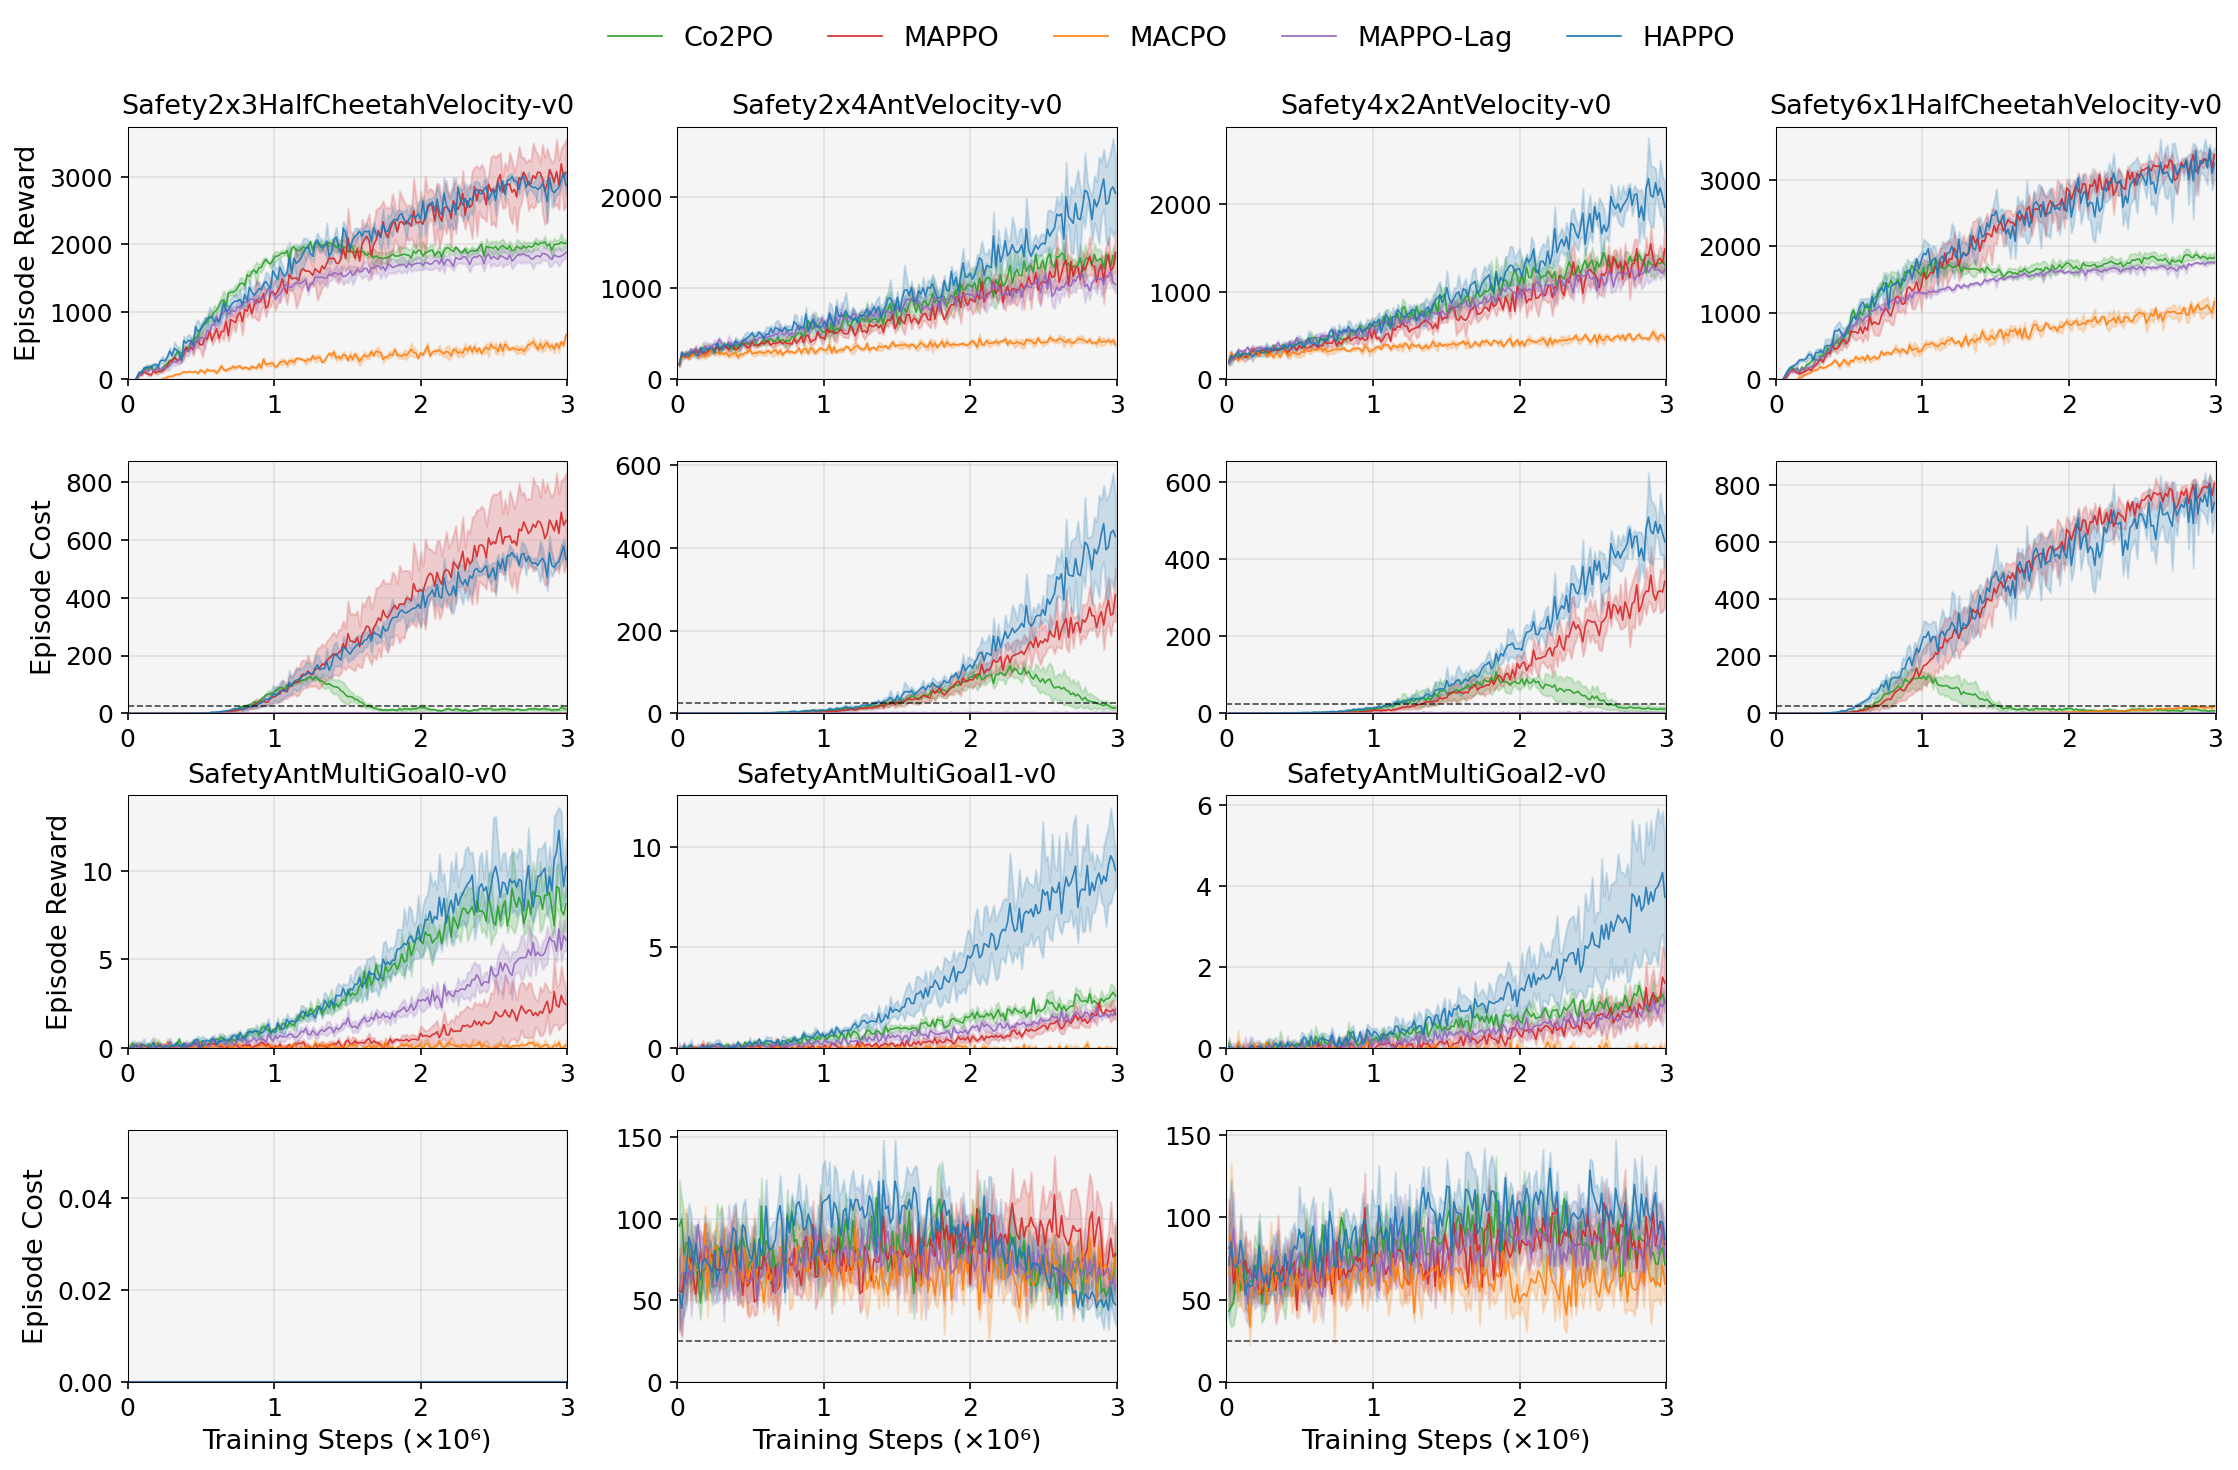
\includegraphics[width=0.99\textwidth]{results_new.png}
  \caption{%
Results on seven \textsc{SafePO} cooperative safety benchmarks.
We report both evaluation return and cost.
  }
  \label{fig:co2po-results}
\end{figure*}

\section{Results}
We evaluate Co2PO on coordination-intensive environments under constrained multi-agent learning. Across all settings, Co2PO achieves higher feasible returns than leading baselines while maintaining evaluation-time cost compliance at convergence. To facilitate comparison across heterogeneous tasks, we aggregate feasible performance and evaluation-time cost by environment type. 
\label{sec:results}
\begin{table}[h!]
\centering
\caption{Mean feasible return across Velocity and Multi-goal environments, and mean final evaluation cost for Velocity tasks.}
\label{tab:feasible_by_env_type}
\begin{small}
\setlength{\tabcolsep}{4pt}
\begin{tabular}{lccc}
\toprule
\textbf{Method} 
& $\boldsymbol{R_{\text{feas}}}$ (Vel.) 
& $\boldsymbol{R_{\text{feas}}}$ (Multi.) 
& $\boldsymbol{C_{\text{final}}}$ (Vel.) \\
\midrule
MAPPO 
& $866$ 
& $3.38$ 
& $525.34$ \\
MAPPO-Lag 
& $1593$ 
& $7.09$ 
& $1.54$ \\
MACPO 
& $738$ 
& $0.69$ 
& $6.94$ \\
HAPPO 
& $1023$ 
& $13.00$ 
& $536.05$ \\
\midrule
\textbf{Co2PO} 
& $\boldsymbol{1709}$ 
& $\boldsymbol{10.00}$ 
& $\boldsymbol{12.30}$ \\
\bottomrule
\end{tabular}
\end{small}
\end{table}



\subsection{Feasible Performance Under Safety Constraints}
\label{sec:feasible}
Co2PO consistently identifies higher-quality feasible solutions throughout training. 
Across velocity-based environments, Co2PO achieves a mean feasible-return improvement of approximately $7\%$ relative to MAPPO-Lag, with a median improvement of $7\%$ (\cref{tab:feasible_by_env_type}). 
These gains are consistent across all velocity tasks, ranging from $6.5\%$ to $7.9\%$ depending on the environment.

In the coordination-intensive multi-goal environment with a feasible region, Co2PO achieves an absolute feasible-return improvement of $2.91$ over MAPPO-Lag (see Appendix~\ref{app:results} for all per-environment statistics). Although the percentage gains are inflated by small baseline values, the absolute improvement confirms Co2PO’s effectiveness in coordination-heavy regimes.


Co2PO demonstrates consistent deployment readiness on the Velocity family: final evaluation costs stabilize across seeds, and cost-compliant checkpoints are reliably reached while maintaining strong returns. 
In all MultiGoal settings, no method reaches the cost budget within the training horizon, so we focus on return--cost tradeoffs rather than feasible return (\cref{sec:ablations}).

\subsection{Learning Dynamics and Exploration--Safety Tradeoff}
\begin{table}[h!]
  \caption{Mean early return and peak episodic cost for velocity environments.}
  \label{tab:exploration_safety_tradeoff}
  \centering
  \begin{small}
  \setlength{\tabcolsep}{6pt}
  \begin{tabular}{l c c}
    \toprule
    \textbf{Method} & $\boldsymbol{C_{\text{peak}}}$ (Vel.) & $\boldsymbol{R_{\text{early}}}$ (Vel.) \\
    \midrule
    MAPPO & $855$ & $1023$ \\
    MAPPO-Lag & $2$ & $881$ \\
    MACPO & $79$ & $622$ \\
    HAPPO & $792$ & $1124$ \\
    \midrule
    \textbf{Co2PO} & $\boldsymbol{231}$ & $\boldsymbol{1221}$ \\
    \bottomrule
  \end{tabular}
  \end{small}
  \vskip -0.08in
\end{table} 


Peak episodic cost $C_{\text{peak}}$ characterizes worst-case constraint violations during training and highlights differences in exploration behavior. 
Co2PO permits bounded early violations, incurring higher peak cost than conservative constrained baselines while remaining substantially below unconstrained methods (\cref{tab:exploration_safety_tradeoff}). 
This behavior is confined to early training and reflects an intentional relaxation of constraint enforcement to promote exploration.

This relaxation enables faster reward acquisition. 
Over the first $10^6$ environment steps, Co2PO achieves higher early evaluation return than MAPPO-Lag and MACPO, indicating more rapid learning progress under partial observability. 
In contrast, methods that aggressively suppress early violations exhibit lower peak cost but slower reward growth and ultimately converge to lower feasible return (\cref{sec:feasible}). 
By tolerating transient violations while enforcing constraints at convergence, Co2PO accelerates learning toward higher-quality, deployable policies.


\subsection{Deployment Safety and Stability}

We evaluate deployment safety using final evaluation cost $C_{\text{final}}$ and violation statistics at convergence. 
Across velocity environments, Co2PO exhibits stable and bounded cost behavior at evaluation time, with low variation across tasks (coefficient of variation, CV $\approx 0.20$), indicating predictable deployment performance. This stability is comparable to that of constrained baselines (MAPPO-Lag CV $\approx 0.29$, MACPO CV $\approx 1.53$), showing that Co2PO’s constraint satisfaction generalizes consistently across environments.

Safety constraint satisfaction at convergence is consistent, with a mean standard deviation of approximately $8\%$ across velocity environments. 
Final costs remain within a feasible range (mean $C_{\text{final}} = 12.30$, range $8.85$--$15.17$), indicating reliable constraint enforcement without erratic cost dynamics. The low cost variance, bounded violations, and reliable feasibility attainment indicate that Co2PO’s constraint satisfaction at convergence is consistent and suitable for deployment, rather than brittle or noise-sensitive.

\subsection{Environment-Dependent Behavioral Patterns}

Co2PO’s performance varies systematically with coordination demands. The largest improvements occur in environments requiring explicit multi-agent coordination, such as \textsc{AntVel}, where Co2PO achieves substantially higher feasible return and more reliable constraint satisfaction than constrained baselines ($R_{\text{feas}} \approx 1{,}450$ vs.\ $\approx 1{,}350$ for MAPPO-Lag across \textsc{AntVel} environments; Appendix~\ref{app:results}). In these settings, reactive and unconstrained baselines frequently fail to converge to compliant solutions within the training horizon: MAPPO and HAPPO do not achieve feasibility in all of the environments, including \textsc{HalfCheetahVel} variants. 

In contrast, environments with simpler dynamics and weaker inter-agent coupling, such as single-direction \textsc{HalfCheetahVel} variants, exhibit more modest but consistent gains ($R_{\text{feas}} \approx 1{,}950$ vs.\ $\approx 1{,}850$), while maintaining comparable stability at convergence. A similar trend appears in multi-goal environments, where Co2PO yields large relative improvements (approximately $40\%$ over MAPPO-Lag; Appendix~\ref{app:results}). Overall, Co2PO’s benefits are environment-dependent rather than uniform, scaling with coordination demands while generalizing across diverse tasks.


\subsection{Comparative Safety–Performance Analysis}

The evaluated baselines exhibit distinct safety--performance tradeoffs. 
Unconstrained methods such as HAPPO and MAPPO achieve high returns but incur substantial costs and elevated violation rates. 
MAPPO-Lag reliably enforces constraints but converges to overly conservative policies, resulting in markedly reduced feasible return. 
MACPO occupies an intermediate regime, mitigating some violations while allowing limited exploration, but consistently underperforms Co2PO across all evaluated environments.

Co2PO differs by enabling proactive constraint enforcement. 
Through hazard prediction and selective inter-agent communication, Co2PO permits controlled early exploration without sacrificing constraint satisfaction at convergence.
This yields a consistently improved safety--performance tradeoff, combining both higher feasible return and reliable deployment-time safety.

Overall, these results suggest that coupling selective coordination with predicted risk provides a practical mechanism for balancing exploration and constraint satisfaction. Importantly, Co2PO’s gains do not stem from constraint enforcement alone, but from improved coordination efficiency that allows agents to reach higher feasible returns.

%%%%%%%%%%%%%%%%%%%%%%%%%%%%%%%%%%%%%%%%%%%%%%%%%%%%%%%%%%%%%%%%%%%%%%%%%%%%%
\section{Ablations}
\label{sec:ablations}

\begin{figure*}[h!]
  \centering
  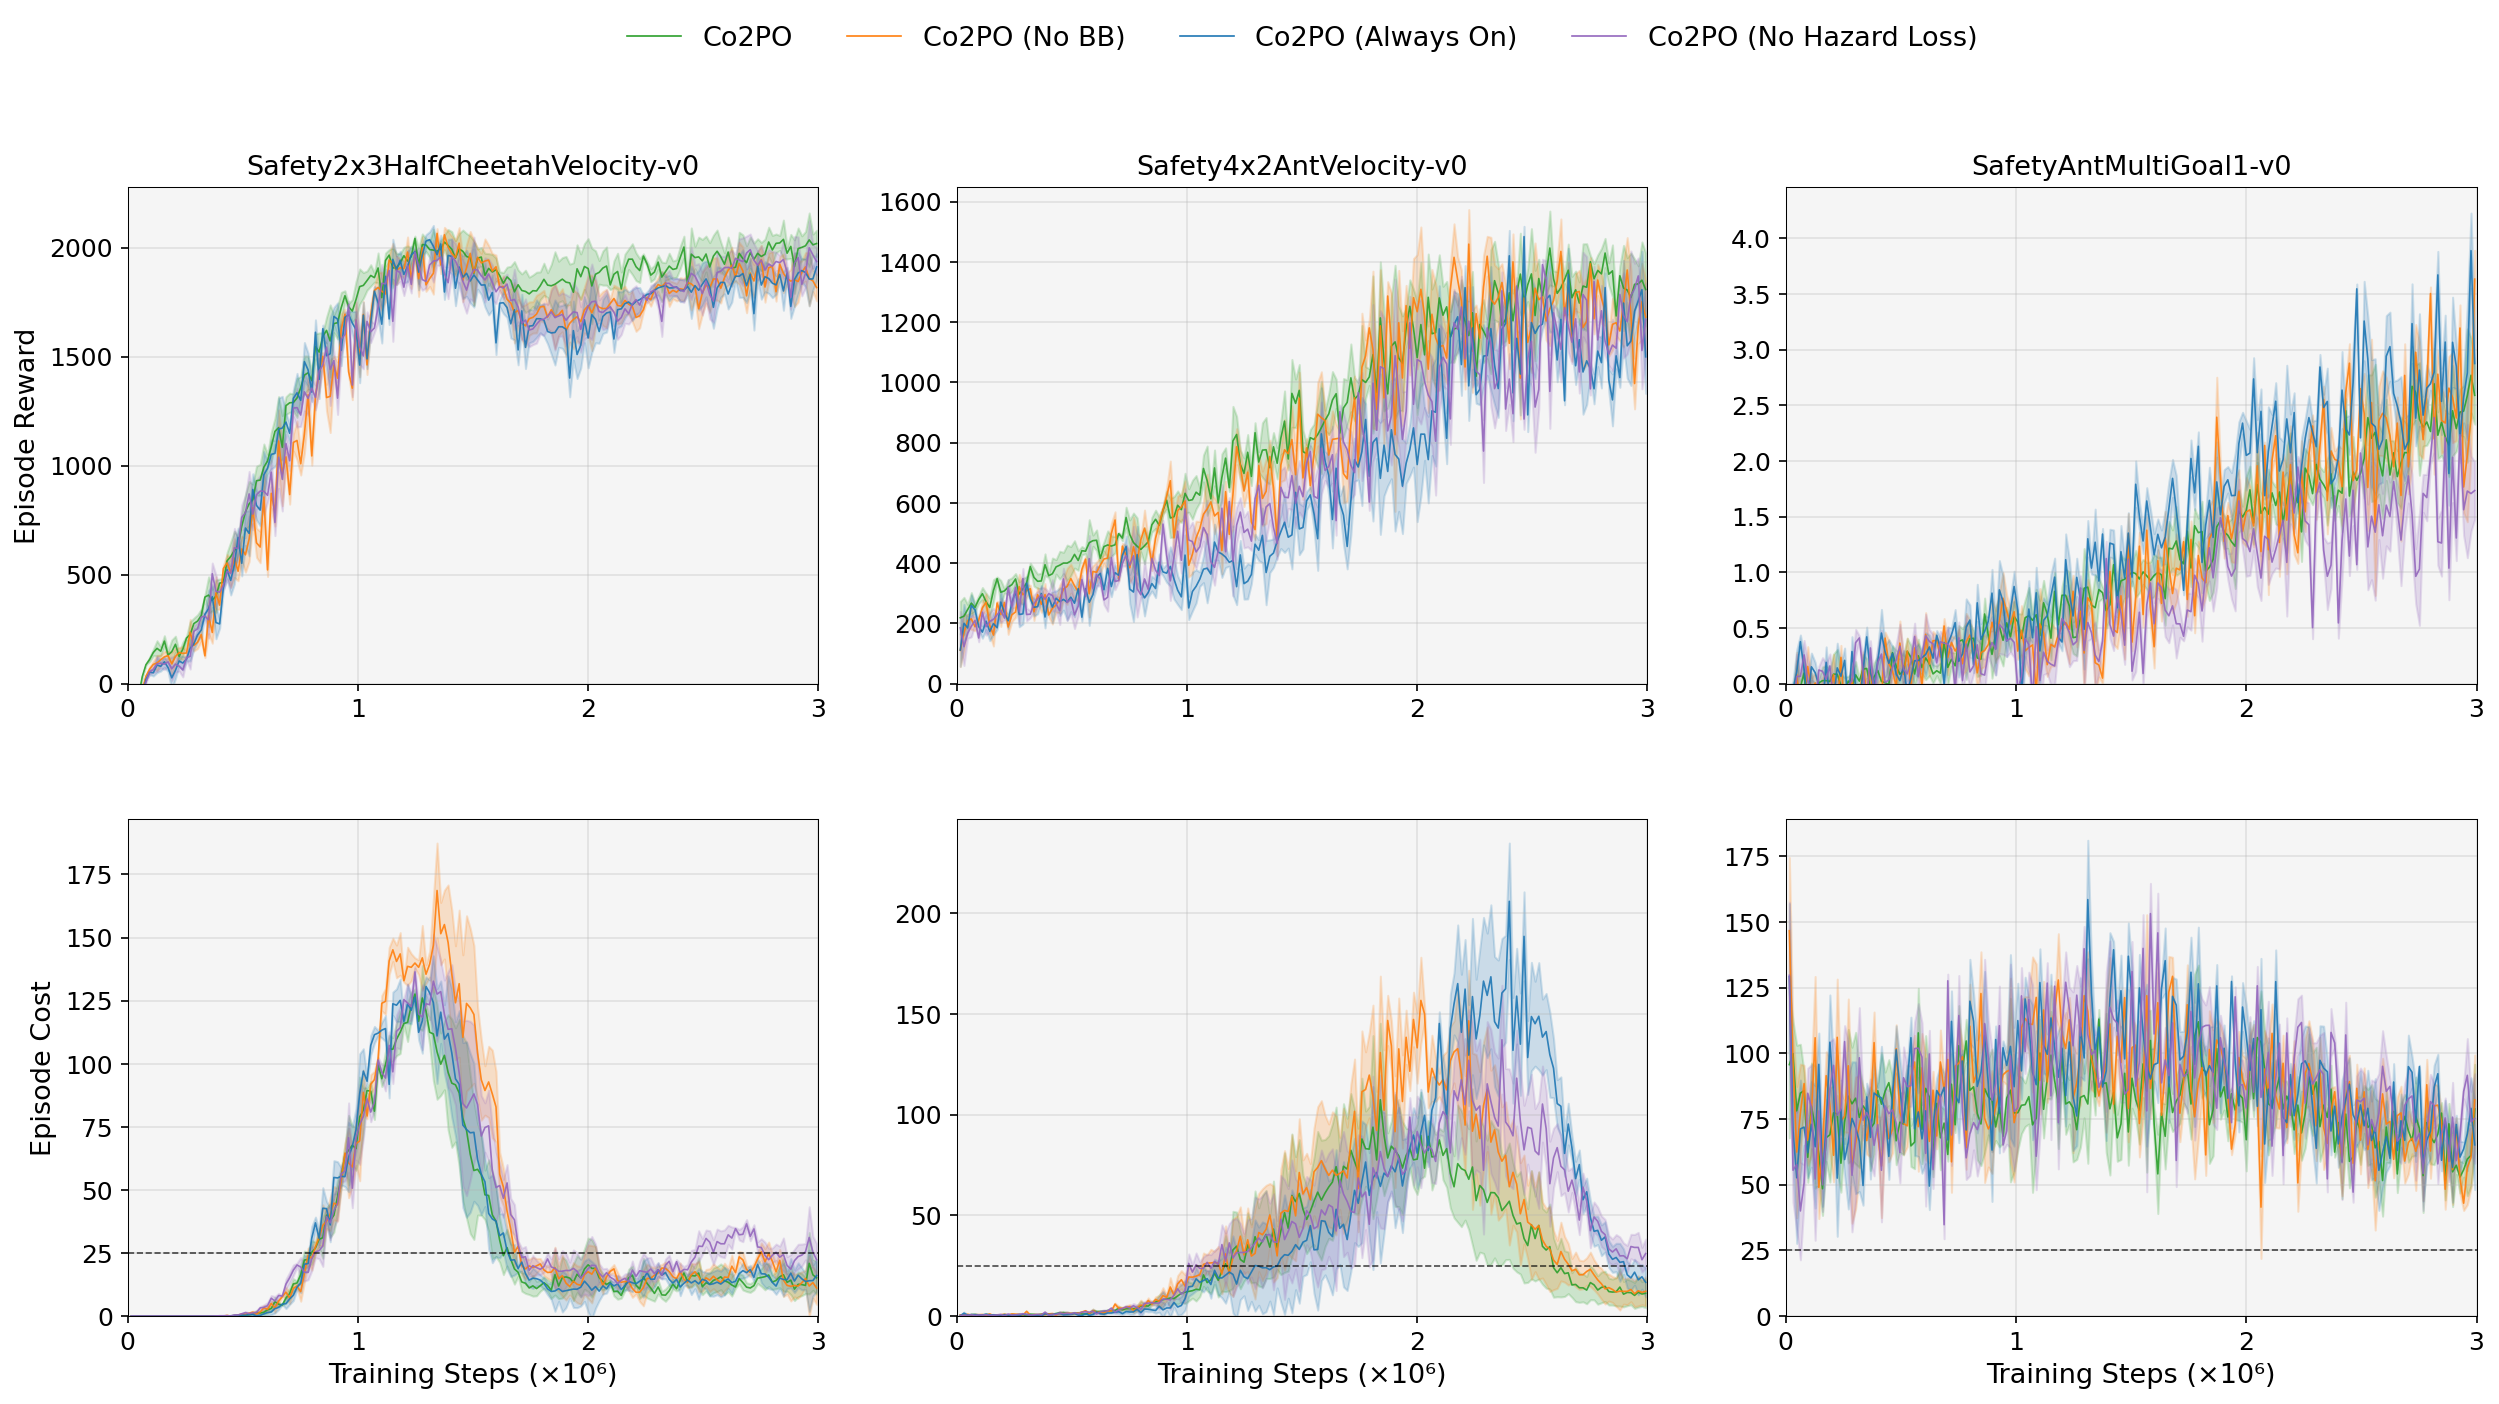
\includegraphics[width=0.99\textwidth]{co2po_ablations.png}
  \caption{%
    Ablations on three environments. We report both evaluation return and cost.
  }
  \label{fig:co2po-ablations}
\end{figure*}

\begin{table*}[h!]
\centering
\small
\setlength{\tabcolsep}{4pt}
\caption{\textbf{Ablation summary.} For Velocity tasks we report \emph{feasible return} and the final evaluation cost $C_{\mathrm{final}}$ at the last checkpoint.
For \textsc{AntMultiGoal}, no method reaches the budget within the plotted horizon, so we report final return $R_{\mathrm{final}}$ instead.}
\label{tab:ablation_co2po}
\begin{tabular}{lcccccc}
\toprule
& \multicolumn{2}{c}{HalfCheetahVel} & \multicolumn{2}{c}{AntVel} & \multicolumn{2}{c}{AntMultiGoal} \\
\cmidrule(lr){2-3}\cmidrule(lr){4-5}\cmidrule(lr){6-7}
\textbf{Method} &
$R_{\mathrm{feas}}\uparrow$ & $C_{\mathrm{final}}\downarrow$ &
$R_{\mathrm{feas}}\uparrow$ & $C_{\mathrm{final}}\downarrow$ &
$R_{\mathrm{final}}\uparrow$ & $C_{\mathrm{final}}\downarrow$ \\
\midrule
\textsc{Co2PO} & 2054 $\pm$ 70 & 15.2 $\pm$ 7.9 & 1468 $\pm$ 43 & 11.3 $\pm$ 8.8 & 2.59 $\pm$ 0.32 & 78.8 $\pm$ 20.8 \\
\textsc{Co2PO} w/o Blackboard & 1907 $\pm$ 65 & 12.3 $\pm$ 6.4 & 1365 $\pm$ 40 & 13.7 $\pm$ 10.6 & 3.46 $\pm$ 0.42 & 84.4 $\pm$ 22.3 \\
\textsc{Co2PO} (Always-Write) & 1915 $\pm$ 65 & 16.6 $\pm$ 8.6 & 1284 $\pm$ 38 & 14.9 $\pm$ 11.6 & 3.07 $\pm$ 0.38 & 67.0 $\pm$ 17.7 \\
\textsc{Co2PO} w/o Hazard Loss & 1936 $\pm$ 66 & 23.1 $\pm$ 12.0 & 566 $\pm$ 17 & 28.2 $\pm$ 21.9 & 1.98 $\pm$ 0.24 & 74.6 $\pm$ 19.7 \\
\bottomrule
\end{tabular}
\end{table*}

We ablate Co2PO's coordination components to isolate which mechanisms drive improvements in feasible performance.
We focus on three representative environments that span fast locomotion with interaction-driven hazards (\textsc{HalfCheetahVel}, \textsc{AntVel}) and a harder navigation-and-coordination setting (\textsc{AntMultiGoal}).
All ablations keep the same training budget and settings as the full method. We additionally study the effect of the hazard lookahead horizon in Appendix~\ref{app:lookahead}.

\textbf{Takeaway.}
\cref{fig:co2po-ablations,tab:ablation_co2po} shows that removing \emph{either} (i) shared-memory coordination (\emph{w/o Blackboard}) or (ii) selective gating (\emph{Always-Write}) reduces feasible performance on the Velocity tasks.
The most pronounced degradation occurs when removing hazard supervision (\emph{w/o Hazard Loss}), which substantially worsens both feasibility and performance in \textsc{AntVel}.

\subsection{Shared Memory Is Beneficial for Feasible Performance}
\label{sec:ablate-blackboard}

\textbf{w/o Blackboard} removes inter-agent shared context, while keeping the rest of training unchanged.
On \textsc{HalfCheetahVel} and \textsc{AntVel}, this consistently lowers feasible return relative to Co2PO (e.g., $2054\!\rightarrow\!1907$ on \textsc{HalfCheetahVel} and $1468\!\rightarrow\!1365$ on \textsc{AntVel}), indicating that the blackboard context is contributing useful coordination information beyond what is recoverable from local observations alone.
Final evaluation costs remain below budget in these Velocity settings, suggesting the main effect of removing the blackboard is reduced \emph{feasible performance} rather than purely increased constraint violations.

In \textsc{AntMultiGoal}, none of the compared methods reaches the budget within the plotted horizon; we therefore report final return instead of feasible return.
Here, removing the blackboard increases $R_{\mathrm{final}}$ but also increases $C_{\mathrm{final}}$ (Table~\ref{tab:ablation_co2po}), highlighting that this environment exhibits a different trade-off regime where constraint satisfaction is not yet achieved by any method in the training budget we consider.

\subsection{Selective Writes Matter}
\label{sec:ablate-always-write}

\textbf{Always-Write} disables sparsity by forcing all agents to write every timestep, while keeping the same message format and read mechanism.
Across the Velocity tasks, Always-Write underperforms the full method in feasible return (e.g., $2054\!\rightarrow\!1915$ on \textsc{HalfCheetahVel} and $1468\!\rightarrow\!1284$ on \textsc{AntVel}), with final costs that remain broadly comparable.
This supports the practical motivation for selective coordination: indiscriminate writing does not reliably improve feasible performance under a fixed training budget, and can introduce additional noise into the retrieved context.

On \textsc{AntMultiGoal}, Always-Write yields a lower final cost than the full method but does not resolve infeasibility; all variants remain above the budget.
We treat this setting as a stress test as none of the baselines reach compliance with regard to the set cost target.

\subsection{Hazard Supervision Is Important for Feasibility}
\label{sec:ablate-hazard}

\textbf{w/o Hazard Loss} removes explicit supervision of the hazard predictor while leaving the coordination pathway intact.
This ablation has the most severe impact on \textsc{AntVel}: feasible return collapses ($1468\!\rightarrow\!566$) and final cost rises above the budget ($11.3\!\rightarrow\!28.2$).
The learning curves in \cref{fig:co2po-ablations} are consistent with the intuition that without direct hazard learning signal, the write trigger becomes less aligned with safety-relevant events, reducing the effectiveness of selective coordination and degrading constraint satisfaction.

On \textsc{HalfCheetahVel}, the same ablation increases final cost while still remaining under budget on average (Table~\ref{tab:ablation_co2po}), and yields a modest drop in feasible return relative to the full method.
On \textsc{AntMultiGoal}, removing hazard supervision decreases final return without materially changing the overall infeasibility regime.


%%%%%%%%%%%%%%%%%%%%%%%%%%%%%%%%%%%%%%%%%%%%%%%%%%%%%%%%%%%%%%%%%%%%%%%%%%%%%%
\section{Related Work}
\label{sec:related}

\textbf{Constrained Reinforcement Learning.}
Constrained reinforcement learning (CRL) addresses policy optimization under explicit safety, resource, or performance constraints, most commonly via Lagrangian relaxation that embeds costs into the objective through adaptive penalty coefficients \cite{zhang2019marlsurvey}.
Single-agent methods such as CPO \cite{achiam2017constrainedpolicyoptimization}, PPO with Lagrangian relaxation \cite{ray2019safexp}, and FOCOPS \cite{zhang2020orderconstrainedoptimizationpolicy} enforce constraints in expectation, but are often sensitive to penalty tuning and rely on reactive updates that correct violations only after they occur, which can slow learning or induce conservative behavior \cite{stooke2020responsive}.
Extensions to multi-agent settings adopt similar principles, employing centralized critics or shared multipliers (e.g., MAPPO-Lagrangian and MACPO) to enforce global constraints.
While effective at reducing violations, these approaches largely rely on reactive, penalty-based constraint handling and can suppress exploration in coordination-intensive environments.


\textbf{Safe Multi-Agent Reinforcement Learning.} Safe multi-agent reinforcement learning (Safe MARL) further considers cooperative settings where safety violations arise from collective interactions rather than isolated actions. Most safe MARL methods operate under the centralized training with decentralized execution (CTDE) paradigm and augment standard MARL backbones such as MAPPO with global cost critics or shared constraint signals \cite{hernandezleal2019surveylearningmultiagentenvironments, foerster2024counterfactualmultiagentpolicygradients}, rather than value-factorization approaches such as QMIX \cite{sunehag2017valuedecompositionnetworkscooperativemultiagent, rashid2018qmixmonotonicvaluefunction}. However, safety is typically enforced through aggregated penalties that provide limited guidance for resolving coordination-induced violations, leading to slow learning dynamics or overly conservative policies \cite{gu2023macpo}. Prior work in hierarchical MARL demonstrates that explicit coordination improves task performance, suggesting that similar mechanisms may be beneficial for safety-constrained multi-agent settings.



\textbf{Communication and Memory in MARL.} Communication has been widely studied as a means of improving coordination in MARL, particularly under partial observability, through message passing or graph-based information sharing \cite{sukhbaatar2016learningmultiagentcommunicationbackpropagation, kim2019schednet, das2020tarmactargetedmultiagentcommunication, jiang2020graphconvolutionalreinforcementlearning}.
Existing approaches primarily use communication to enhance task performance and learning stability 
\cite{peng2021copo,calzolari2026safeheterogeneousmultiagentrl}, without explicitly targeting safety constraints. Some methods combine communication with safety mechanisms by coupling MAPPO-style training with execution-time safety filters or shields \cite{alshiekh2017safereinforcementlearningshielding}, while others incorporate shared cost signals during training to enforce constraints.
In both cases, safety is handled reactively via centralized penalties or post-hoc intervention, and communication is rarely conditioned on anticipated risk or collective hazard.

Co2PO departs from prior work by coupling communication with safety objectives as part of the learning process, rather than engineering safety as an external rule. In addition to Lagrangian constraint penalties, Co2PO leverages hazard prediction to selectively trigger communication and coordination when safety risks are anticipated. Communication is neither constant nor purely performance-driven, but explicitly conditioned on predicted constraint violations, allowing more targeted and efficient safety coordination.




%%%%%%%%%%%%%%%%%%%%%%%%%%%%%%%%%%%%%%%%%%%%%%%%%%%%%%%%%%%%%%%%%%%%%%
\section{Discussion}
\label{sec:conclusion}

\textbf{Why Co2PO helps.}
Our central hypothesis is that many safety failures in cooperative MARL are \emph{coordination-induced}: violations arise from mismatched timing, intent, or mutual awareness under partial observability. Co2PO addresses this by turning communication into a \emph{risk-triggered control signal}. Agents only broadcast when their hazard predictor anticipates near-term risk, and the blackboard carries compact, safety-relevant semantics (state summary, intent, yield, hazard probability) that other agents can immediately condition on. This differs from purely reactive constraint handling, where penalties increase \emph{after} violations and can suppress exploration globally \cite{brunke2022safelearning, gu2023macpo}.


\textbf{Empirical takeaways.}
Across seven \textsc{SafePO} benchmarks, Co2PO consistently finds higher-quality feasible checkpoints than strong constrained baselines, especially on the Velocity family where interaction-driven hazards are common (\cref{fig:co2po-results}). The learning curves also reflect an explicit exploration--safety strategy: Co2PO tolerates bounded early violations (higher $C_{\text{peak}}$) to acquire reward faster, then improves constraint satisfaction and stabilizes by deployment (\cref{sec:results}). Ablations isolate the key mechanisms, justifying the role of the blackboard, selective writes, and hazard supervision (\cref{fig:co2po-ablations,tab:ablation_co2po}). In the appendix, varying the lookahead horizon further supports the role of proactive labeling as nonzero horizons can improve the return--cost tradeoff relative to $H\!=\!0$ (\cref{app:lookahead}).

\textbf{Limitations and future work.}
First, Co2PO is designed to target \emph{deployment-safe policies under a fixed training budget}, rather than zero-violation training-time safety \cite{alshiekh2017safereinforcementlearningshielding, berkenkamp2017safemodelbasedreinforcementlearning}: peak violations can be larger than conservative baselines, which may be unacceptable in some real systems.
Second, our hazard labels rely on dense per-step costs and a hand-chosen threshold $\delta$ (and horizon $H$), which may not be available or stable across domains; learning hazard signals from sparse events, uncertainty-aware predictors, or model-based rollouts is a natural extension \cite{yang2020meanfieldmultiagentreinforcement, calzolari2026safeheterogeneousmultiagentrl}. Third, the Multi-Goal regime remains challenging under our fixed budget, suggesting we need training signals that better reflect delayed coordination effects (e.g., when early yielding prevents later conflicts). Finally, we have not yet stressed scalability: blackboard retrieval and message semantics may need compression, structured routing, or graph-based selection as agent counts grow \cite{goeckner2024graphbasedmar}. Together, these directions would broaden Co2PO’s applicability and improve robustness of risk-triggered coordination across domains, horizons, and agent scales.

\clearpage

%%%%%%%%%%%%%%%%%%%%%%%%%%%%%%%%%%%%%%%%%%%%%%%%%%%%%%%%%%%%%%%%%%%%%%%%%%%%%%%
% Acknowledgements (ONLY in accepted version):
% \section*{Acknowledgements}
% TODO

%%%%%%%%%%%%%%%%%%%%%%%%%%%%%%%%%%%%%%%%%%%%%%%%%%%%%%%%%%%%%%%%%%%%%%%%%%%%%%%
% Impact Statement (required by ICML):
\section*{Impact Statement}
This work advances methods for learning policies under safety constraints in multi-agent environments. Improved constrained MARL can reduce unsafe behavior in high-stakes domains where multiple decision-makers interact. Potential risks include misuse in adversarial settings or deployment without adequate monitoring; we encourage careful evaluation, transparent reporting of training-time violations, and robust safety testing prior to real-world use.

%%%%%%%%%%%%%%%%%%%%%%%%%%%%%%%%%%%%%%%%%%%%%%%%%%%%%%%%%%%%%%%%%%%%%%%%%%
\bibliographystyle{icml2026}
\bibliography{citations}
\clearpage

%%%%%%%%%%%%%%%%%%%%%%%%%%%%%%%%%%%%%%%%%%%%%%%%%%%%%%%%%%%%%%%%%%%%%%

% APPENDIX

\newpage
\appendix
\section{Complete Evaluation Metrics}
\label{app:results}

\begin{table}[h!]
\centering
\caption{Full evaluation metrics aggregated across runs.}
\label{tab:full_metrics}
\resizebox{\textwidth}{!}{
\begin{tabular}{llcccccc}
\toprule
\textbf{Environment} & \textbf{Method} & $\boldsymbol{R_{\text{final}}}$ & $\boldsymbol{R_{\text{feas}}}$ & $\boldsymbol{C_{\text{final}}}$ & $\boldsymbol{C_{\text{peak}}}$ & \textbf{Violation rate} & \textbf{Time-to-feasible} \\
\midrule
\multirow{5 }{* }{}{Safety2x3HalfCheetahVelocity} & MAPPO & $3068 \pm 491$ & $1094 \pm 43$ & $667.17 \pm 164.13$ & $712$ & $0.71 \pm 0.02$ & -- \\
 & MAPPO-Lag & $1882 \pm 74$ & $1904 \pm 86$ & $1.10 \pm 0.51$ & $3$ & $0.00 \pm 0.00$ & $16000$ \\
 & MACPO & $657 \pm 22$ & $663 \pm 16$ & $0.48 \pm 0.21$ & $0$ & $0.00 \pm 0.00$ & $16000$ \\
 & HAPPO & $2878 \pm 143$ & $1362 \pm 95$ & $532.04 \pm 21.41$ & $583$ & $0.72 \pm 0.02$ & -- \\
 & \textbf{Co2PO} & $\mathbf{2018 \pm 61}$ & $\mathbf{2054 \pm 57}$ & $\mathbf{15.17 \pm 6.46}$ & $\mathbf{133}$ & $\mathbf{0.30 \pm 0.01}$ & $\mathbf{1704000}$ \\
\midrule
\multirow{5 }{* }{}{Safety2x4AntVelocity} & MAPPO & $1386 \pm 242$ & $704 \pm 37$ & $286.34 \pm 64.61$ & $305$ & $0.50 \pm 0.04$ & -- \\
 & MAPPO-Lag & $1038 \pm 89$ & $1315 \pm 51$ & $1.39 \pm 0.52$ & $3$ & $0.00 \pm 0.00$ & $16000$ \\
 & MACPO & $378 \pm 29$ & $493 \pm 22$ & $0.53 \pm 0.28$ & $1$ & $0.00 \pm 0.00$ & $16000$ \\
 & HAPPO & $2041 \pm 405$ & $933 \pm 60$ & $427.80 \pm 99.41$ & $494$ & $0.54 \pm 0.02$ & -- \\
 & \textbf{Co2PO} & $\mathbf{1330 \pm 41}$ & $\mathbf{1418 \pm 42}$ & $\mathbf{13.82 \pm 4.80}$ & $\mathbf{133}$ & $\mathbf{0.45 \pm 0.04}$ & $\mathbf{2810667}$ \\
\midrule
\multirow{5 }{* }{}{Safety4x2AntVelocity} & MAPPO & $1486 \pm 254$ & $698 \pm 38$ & $341.95 \pm 65.31$ & $383$ & $0.55 \pm 0.03$ & -- \\
 & MAPPO-Lag & $1253 \pm 103$ & $1374 \pm 92$ & $1.47 \pm 0.64$ & $4$ & $0.00 \pm 0.00$ & $16000$ \\
 & MACPO & $459 \pm 20$ & $559 \pm 22$ & $1.47 \pm 0.66$ & $2$ & $0.00 \pm 0.00$ & $16000$ \\
 & HAPPO & $1966 \pm 290$ & $749 \pm 42$ & $444.63 \pm 67.31$ & $570$ & $0.61 \pm 0.02$ & -- \\
 & \textbf{Co2PO} & $\mathbf{1308 \pm 121}$ & $\mathbf{1468 \pm 35}$ & $\mathbf{11.34 \pm 7.19}$ & $\mathbf{126}$ & $\mathbf{0.42 \pm 0.03}$ & $\mathbf{2528000}$ \\
\midrule
\multirow{5 }{* }{}{Safety6x1HalfCheetahVelocity} & MAPPO & $3381 \pm 4$ & $968 \pm 47$ & $805.90 \pm 9.45$ & $826$ & $0.76 \pm 0.02$ & -- \\
 & MAPPO-Lag & $1754 \pm 15$ & $1778 \pm 16$ & $2.19 \pm 0.98$ & $4$ & $0.00 \pm 0.00$ & $16000$ \\
 & MACPO & $1159 \pm 70$ & $1236 \pm 17$ & $25.29 \pm 2.43$ & $27$ & $0.01 \pm 0.00$ & $2912000$ \\
 & HAPPO & $3249 \pm 238$ & $1047 \pm 35$ & $739.71 \pm 51.41$ & $838$ & $0.82 \pm 0.01$ & -- \\
 & \textbf{Co2PO} & $\mathbf{1829 \pm 79}$ & $\mathbf{1894 \pm 55}$ & $\mathbf{8.85 \pm 4.65}$ & $\mathbf{154}$ & $\mathbf{0.29 \pm 0.04}$ & $\mathbf{1614667}$ \\
\midrule
\multirow{5 }{* }{}{SafetyAntMultiGoal-0} & MAPPO & $2.44 \pm 0.93$ & $3.38 \pm 1.73$ & $0.00 \pm 0.00$ & $0$ & $0.00 \pm 0.00$ & $16000$ \\
 & MAPPO-Lag & $6.08 \pm 0.63$ & $7.09 \pm 0.34$ & $0.00 \pm 0.00$ & $0$ & $0.00 \pm 0.00$ & $16000$ \\
 & MACPO & $0.14 \pm 0.29$ & $0.69 \pm 0.05$ & $0.00 \pm 0.00$ & $0$ & $0.00 \pm 0.00$ & $16000$ \\
 & HAPPO & $10 \pm 1$ & $13 \pm 1$ & $0.00 \pm 0.00$ & $0$ & $0.00 \pm 0.00$ & $16000$ \\
 & \textbf{Co2PO} & $\mathbf{8.13 \pm 1.05}$ & $\mathbf{10 \pm 1}$ & $\mathbf{0.00 \pm 0.00}$ & $\mathbf{0}$ & $\mathbf{0.00 \pm 0.00}$ & $\mathbf{16000}$ \\
\midrule
\multirow{5 }{* }{}{SafetyAntMultiGoal-1} & MAPPO & $1.66 \pm 0.24$ & -- & $78.21 \pm 20.21$ & $137$ & $1.00 \pm 0.00$ & -- \\
 & MAPPO-Lag & $1.93 \pm 0.15$ & -- & $56.30 \pm 7.64$ & $116$ & $1.00 \pm 0.00$ & -- \\
 & MACPO & $-0.12 \pm 0.05$ & -- & $76.46 \pm 5.70$ & $121$ & $1.00 \pm 0.00$ & -- \\
 & HAPPO & $8.84 \pm 0.85$ & -- & $47.38 \pm 12.59$ & $149$ & $1.00 \pm 0.00$ & -- \\
 & \textbf{Co2PO} & $\mathbf{2.59 \pm 0.26}$ & -- & $\mathbf{78.77 \pm 17.02}$ & $\mathbf{135}$ & $\mathbf{1.00 \pm 0.00}$ & -- \\
\midrule
\multirow{5 }{* }{}{SafetyAntMultiGoal-2} & MAPPO & $1.60 \pm 0.72$ & -- & $83.46 \pm 2.57$ & $124$ & $1.00 \pm 0.00$ & -- \\
 & MAPPO-Lag & $1.17 \pm 0.21$ & -- & $76.27 \pm 16.08$ & $127$ & $1.00 \pm 0.00$ & -- \\
 & MACPO & $-0.07 \pm 0.20$ & -- & $59.42 \pm 11.00$ & $122$ & $1.00 \pm 0.00$ & -- \\
 & HAPPO & $3.72 \pm 1.48$ & -- & $86.57 \pm 2.35$ & $151$ & $1.00 \pm 0.00$ & -- \\
 & \textbf{Co2PO} & $\mathbf{1.11 \pm 0.03}$ & -- & $\mathbf{71.27 \pm 0.45}$ & $\mathbf{133}$ & $\mathbf{1.00 \pm 0.00}$ & -- \\
\bottomrule
\end{tabular}
}
\end{table}


%------------------------------------------------------------

\onecolumn

% -----------------------------
% APPENDIX PART FOR LOOKAHEAD!!

\section{Effect of Hazard Lookahead Horizon}
\label{app:lookahead}

We study how the hazard lookahead horizon $H$ used to construct the proactive label $h_t^i$ in \cref{eq:lookahead-hazard} affects final performance. We compare Co2PO variants with $H\!\in\!\{0,3,5,8\}$, using the same training budget ($3{,}000{,}000$ steps) and evaluation protocol. Table~\ref{tab:lookahead} summarizes final-timestep statistics.

Overall, adding a nonzero lookahead yields \emph{consistent} improvements on the coordination-intensive Velocity family: all $H\!>\!0$ variants reduce average final cost relative to $H\!=\!0$ (while slightly increasing average final reward). The clearest improvement appears at the highest horizon ($H\!=\!8$). We also observe that higher horizons increase the number of environments that are cost-compliant at the final checkpoint (from $4/7$ to $5/7$). Longer lookahead ($H\!=\!8$) remains better than $H\!=\!0$ on Velocity costs, but does not further improve the harder MultiGoal settings in our runs (where final costs remain above budget for most methods).

\begin{table}[h!]
\centering
\caption{\textbf{Hazard lookahead horizon $H$ (final-timestep).} We report averages over the four Velocity environments (\textsc{HalfCheetahVel} and \textsc{AntVel}) and the provided averages over all $7$ environments. ``Feasible envs'' counts how many environments satisfy $C_{\text{final}}\le d$ at the final checkpoint (budget $d=25$).}
\label{tab:lookahead}
\small
\setlength{\tabcolsep}{6pt}
\renewcommand{\arraystretch}{1.08}
\begin{tabular}{lcccccc}
\toprule
\textbf{Method} & $\boldsymbol{H}$ &
$\overline{R}_{\text{final}}$ (Vel)$\uparrow$ &
$\overline{C}_{\text{final}}$ (Vel)$\downarrow$ &
\textbf{Feasible envs} $\uparrow$ \\
\midrule
\textsc{Co2PO} & 0 &
1607.79 & 19.34 &
$4/7$ \\
\textsc{Co2PO} & 3 &
1621.88 & 12.30 &
$4/7$ \\
\textsc{Co2PO} & 5 &
1639.69 & 16.32 &

$5/7$ \\
\textsc{Co2PO} & 8 &
1644.18 & 9.42 &

$5/7$ \\
\bottomrule
\end{tabular}
\vspace{-0.5em}
\end{table}

\paragraph{Takeaway.}
These results are consistent with the intuition behind proactive labeling: predicting hazards a few steps ahead provides a cleaner trigger for coordination, improving the safety--performance tradeoff on interaction-driven Velocity tasks.

% -------------------------
% DIAGRAM
% -------------------------
\clearpage
\section{Method Diagram}

\begin{figure*}[h!]
  \centering
  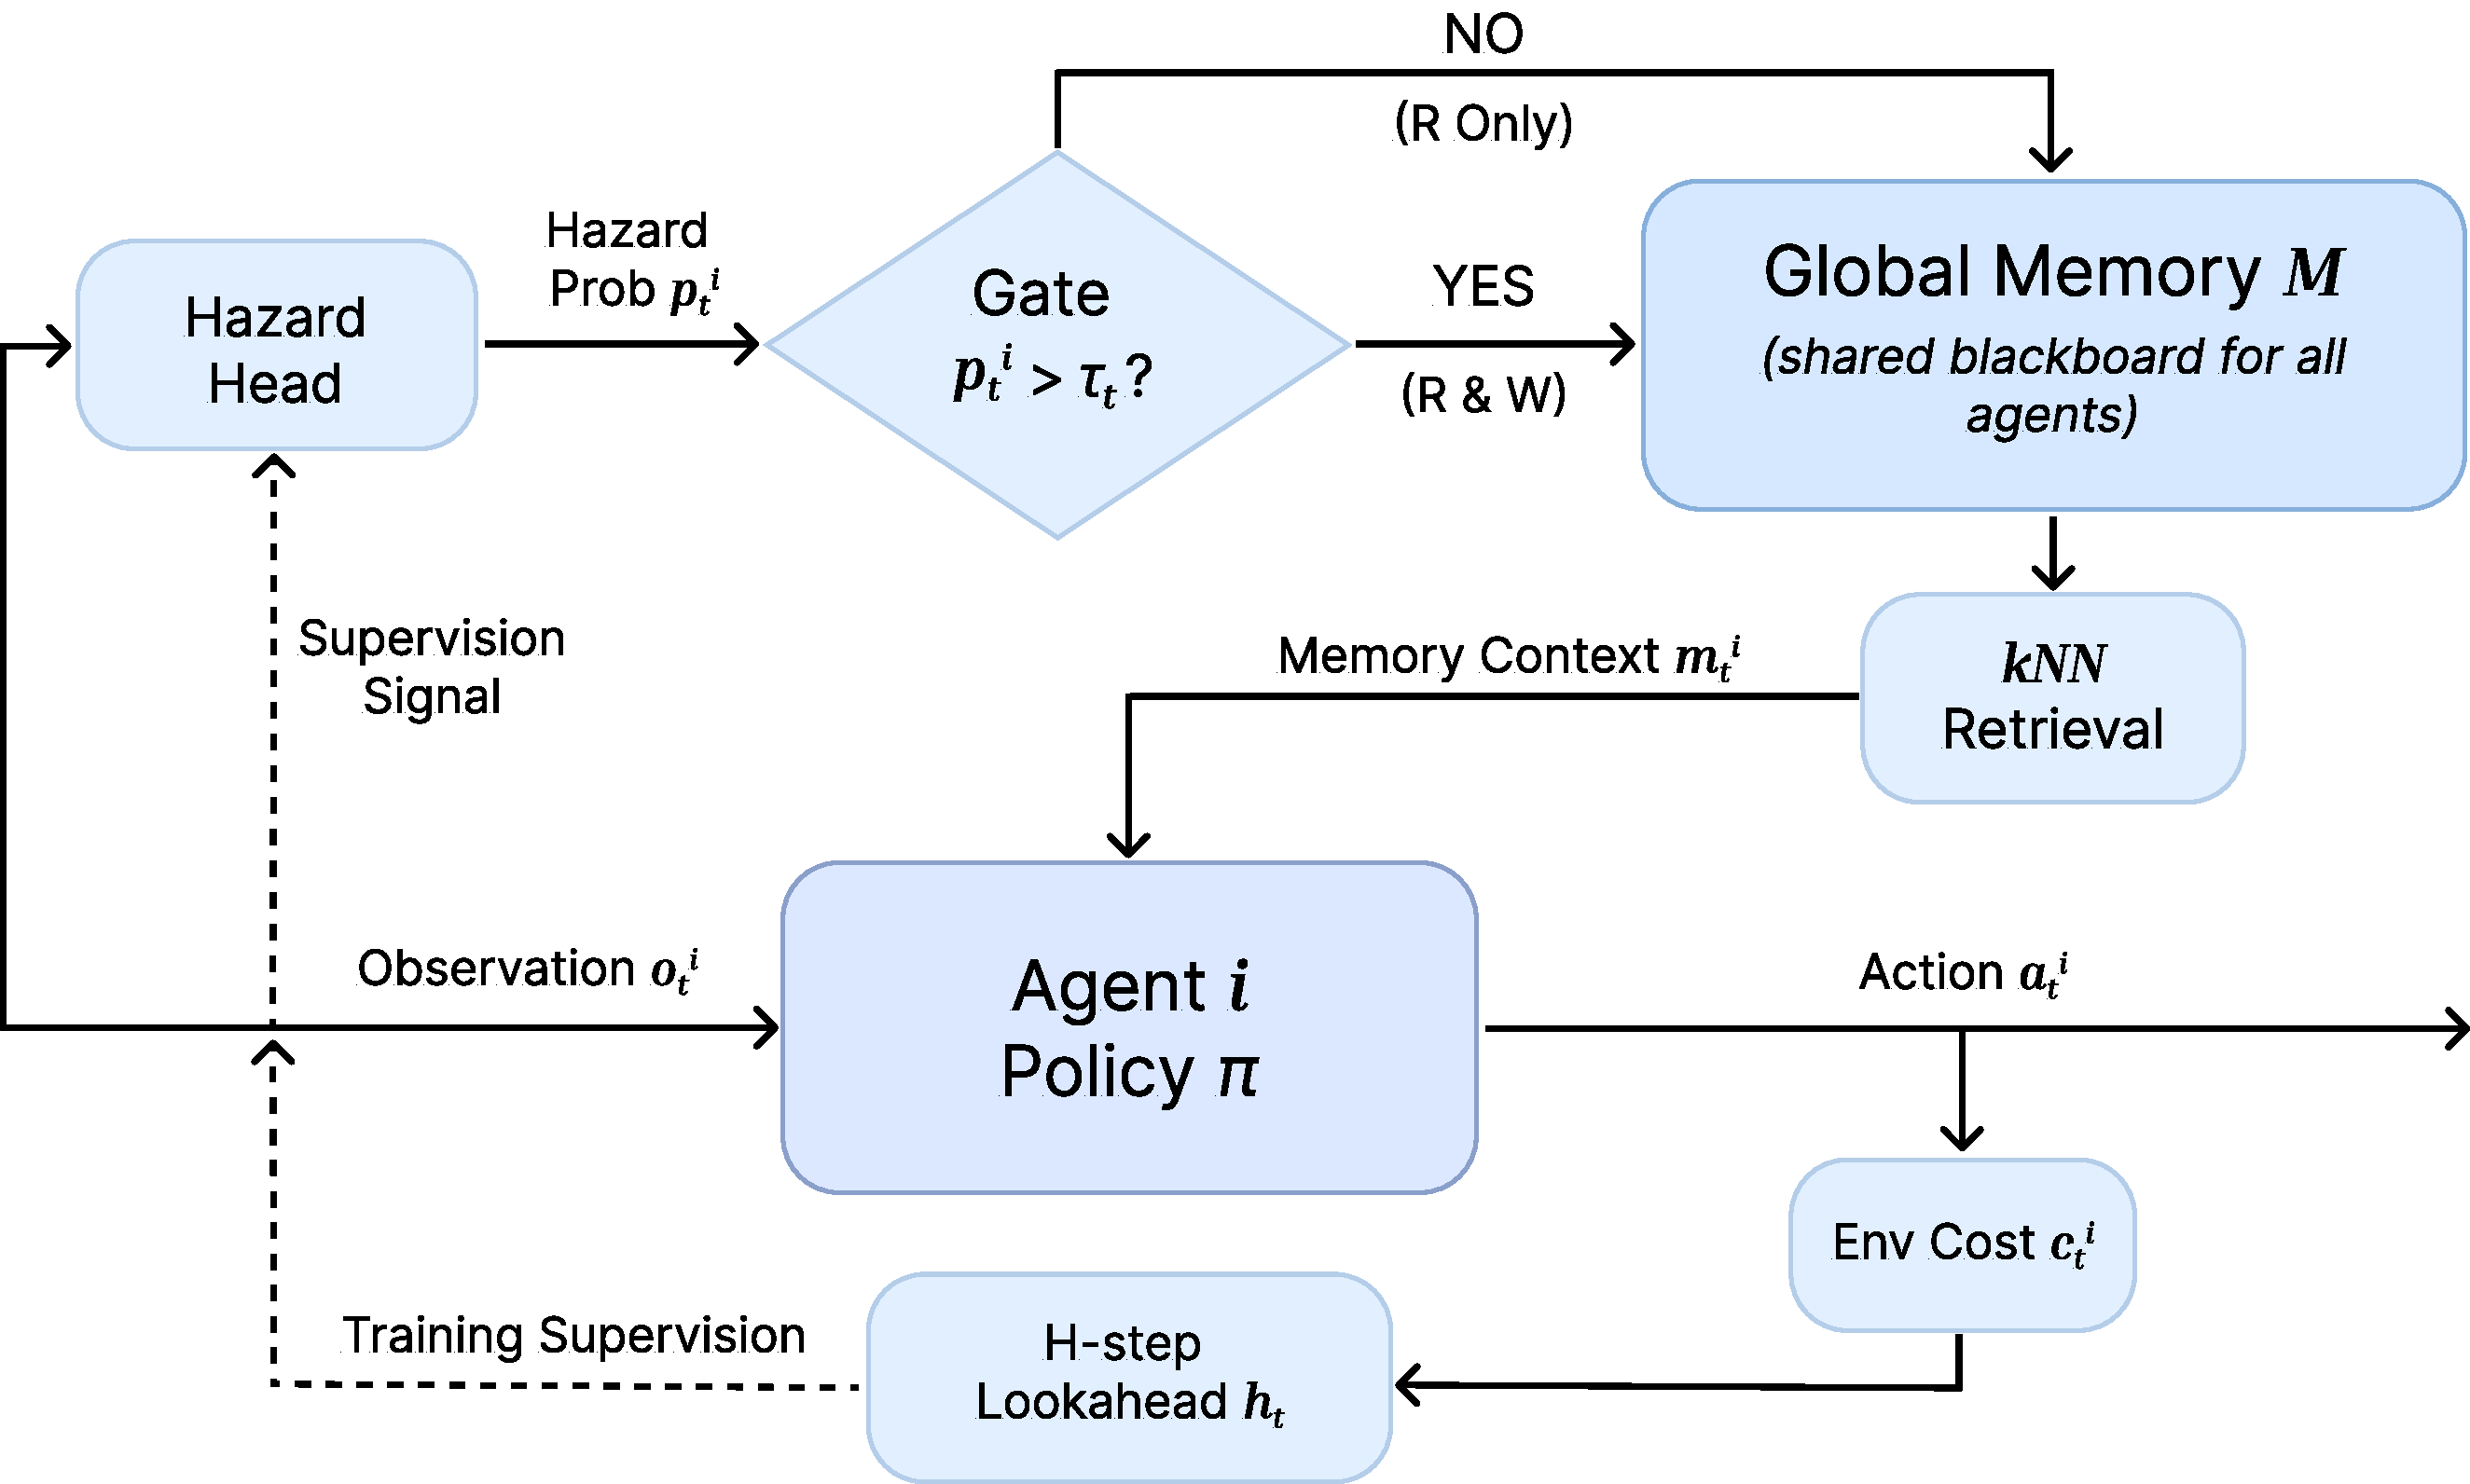
\includegraphics[width=0.87\textwidth]{Co2PO_Diagram.pdf}
  \caption{%
    Co2PO Framework Diagram
  }
  \label{fig:co2po-ablations}
\end{figure*}


% -------------------------
% HYPERPARAM APPENDIX TABLES
% -------------------------
\clearpage
\section{Detailed Hyperparameters}
\label{app:hparams}

\vfill
\begin{table}[h!]
\caption{\textbf{Key method hyperparameters (1/3).} Common run settings are in Table~\ref{tab:common-run-settings}.}
\label{tab:hparams-page1}
\centering
\begin{subtable}[t]{0.48\textwidth}
\caption{\textsc{Co2PO}}
\label{tab:hparams-co2po}
\centering
\scriptsize
\setlength{\tabcolsep}{4pt}
\renewcommand{\arraystretch}{1.08}
\begin{tabular}{@{}p{0.68\linewidth}p{0.26\linewidth}@{}}
\toprule
\textbf{Hyperparameter} & \textbf{Value} \\
\midrule
Hidden size & 256 \\
MLP layers & 2 \\
Discount $\gamma$ & 0.96 \\
GAE $\lambda$ & 0.95 \\
PPO clip $\epsilon$ & 0.2 \\
Target KL & 0.016 \\
Update epochs & 10 \\
Minibatches & 2 \\
Actor LR & $5.0\times 10^{-4}$ \\
Critic LR & $5.0\times 10^{-3}$ \\
Entropy coef. & 0.0 \\
Max grad norm & 10.0 \\
\midrule
Cost budget $d$ & 25 \\
Dual init ($\lambda_0$) & 0.1 \\
Dual step & $5.0\times 10^{-4}$ \\
\midrule
Top-$k$ reads ($k$) & 3 \\
Memory embed dim & 64 \\
Hazard lookahead $H$ & 8 \\
Hazard cost thresh. $\delta$ & 0.1 \\
Write penalty coef. & 0.001 \\
Hazard loss coef. & 0.5 \\
Adaptive threshold & True \\
Init. threshold $\tau$ & 0.10 \\
Target write rate $\rho^\star$ & 0.05 \\
Threshold LR & 0.05 \\
Threshold bounds & [0.05, 0.95] \\
\bottomrule
\end{tabular}
\end{subtable}\hfill
\begin{subtable}[t]{0.48\textwidth}
\caption{\textsc{MAPPO-Lag}}
\label{tab:hparams-mappolag}
\centering
\scriptsize
\setlength{\tabcolsep}{4pt}
\renewcommand{\arraystretch}{1.08}
\begin{tabular}{@{}p{0.68\linewidth}p{0.26\linewidth}@{}}
\toprule
\textbf{Hyperparameter} & \textbf{Value} \\
\midrule
Hidden size & 256 \\
MLP layers & 2 \\
Discount $\gamma$ & 0.96 \\
GAE $\lambda$ & 0.95 \\
PPO clip $\epsilon$ & 0.2 \\
Target KL & 0.016 \\
Update epochs & 10 \\
Minibatches & 2 \\
Actor LR & $9.0\times 10^{-5}$ \\
Critic LR & $5.0\times 10^{-3}$ \\
Entropy coef. & 0.0 \\
Max grad norm & 10.0 \\
\midrule
Cost budget $d$ & 25 \\
Dual init ($\lambda_0$) & 0.78 \\
Dual step & $1.0\times 10^{-5}$ \\
\bottomrule
\end{tabular}
\end{subtable}
\end{table}
\vfill

% -------------------------

\clearpage
\begin{table}[t]
\caption{\textbf{Key method hyperparameters (2/3).} Common run settings are in Table~\ref{tab:common-run-settings}.}
\label{tab:hparams-page2}
\centering
\begin{subtable}[t]{0.48\textwidth}
\caption{\textsc{MAPPO}}
\label{tab:hparams-mappo}
\centering
\scriptsize
\setlength{\tabcolsep}{4pt}
\renewcommand{\arraystretch}{1.08}
\begin{tabular}{@{}p{0.68\linewidth}p{0.26\linewidth}@{}}
\toprule
\textbf{Hyperparameter} & \textbf{Value} \\
\midrule
Hidden size & 256 \\
MLP layers & 2 \\
Discount $\gamma$ & 0.96 \\
GAE $\lambda$ & 0.95 \\
PPO clip $\epsilon$ & 0.2 \\
Target KL & 0.016 \\
Update epochs & 10 \\
Minibatches & 2 \\
Actor LR & $9.0\times 10^{-5}$ \\
Critic LR & $5.0\times 10^{-3}$ \\
Entropy coef. & 0.0 \\
Max grad norm & 10.0 \\
\bottomrule
\end{tabular}
\end{subtable}\hfill
\begin{subtable}[t]{0.48\textwidth}
\caption{\textsc{MACPO}}
\label{tab:hparams-macpo}
\centering
\scriptsize
\setlength{\tabcolsep}{4pt}
\renewcommand{\arraystretch}{1.08}
\begin{tabular}{@{}p{0.68\linewidth}p{0.26\linewidth}@{}}
\toprule
\textbf{Hyperparameter} & \textbf{Value} \\
\midrule
Hidden size & 256 \\
MLP layers & 2 \\
Discount $\gamma$ & 0.96 \\
GAE $\lambda$ & 0.95 \\
PPO clip $\epsilon$ & 0.2 \\
Target KL & 0.016 \\
Update epochs & 10 \\
Minibatches & 2 \\
Actor LR & $9.0\times 10^{-5}$ \\
Critic LR & $5.0\times 10^{-3}$ \\
Entropy coef. & 0.0 \\
Max grad norm & 10.0 \\
\midrule
Cost budget $d$ & 25 \\
Safety $\gamma$ & 0.09 \\
Step fraction & 0.5 \\
CG iters & 10 \\
$g$-step dir coef. & 0.1 \\
$b$-step dir coef. & 0.1 \\
Fraction coef. & 0.1 \\
EPS & $1.0\times 10^{-8}$ \\
\bottomrule
\end{tabular}
\end{subtable}
\end{table}

% -------------------------

\clearpage
\begin{table}[t]
\caption{\textbf{Key method hyperparameters (3/3)} Common run settings listed here.}
\label{tab:hparams-page3}
\centering
\begin{subtable}[t]{0.48\textwidth}
\caption{\textsc{HAPPO}}
\label{tab:hparams-happo}
\centering
\scriptsize
\setlength{\tabcolsep}{4pt}
\renewcommand{\arraystretch}{1.08}
\begin{tabular}{@{}p{0.68\linewidth}p{0.26\linewidth}@{}}
\toprule
\textbf{Hyperparameter} & \textbf{Value} \\
\midrule
Hidden size & 256 \\
MLP layers & 2 \\
Discount $\gamma$ & 0.96 \\
GAE $\lambda$ & 0.95 \\
PPO clip $\epsilon$ & 0.2 \\
Target KL & 0.016 \\
Update epochs & 10 \\
Minibatches & 2 \\
Actor LR & $5.0\times 10^{-4}$ \\
Critic LR & $5.0\times 10^{-4}$ \\
Entropy coef. & 0.0 \\
Max grad norm & 10.0 \\
\bottomrule
\end{tabular}
\end{subtable}\hfill
\begin{subtable}[t]{0.48\textwidth}
\caption{\textbf{Common run settings (all methods)}}
\label{tab:common-run-settings}
\centering
\scriptsize
\setlength{\tabcolsep}{4pt}
\renewcommand{\arraystretch}{1.08}
\begin{tabular}{@{}p{0.68\linewidth}p{0.26\linewidth}@{}}
\toprule
\textbf{Setting} & \textbf{Value} \\
\midrule
Total environment steps & $3{,}000{,}000$ \\
Num parallel environments (\texttt{--num-envs}) & 16 \\
Num seeds (for uncertainty bands) & 3 \\
\bottomrule
\end{tabular}
\end{subtable}
\end{table}




\end{document}
